In this section, we conduct our experiments for four different examples: i) single binary option under discretized GBM model, ii) single call option under discretized GBM model, iii) $2d$-basket call option under discretized GBM model and iv) $4d$-basket call option under discretized GBM model .

For each example, we estimate the weak error  (Bias) of MC, then we conduct a comparison between MC and MISC in terms of errors and computational time. We show tables and plots reporting  the different relative errors involved in the MC method (bias and statistical error\footnote{The statistical error estimate of MC is  $C_{\alpha} \frac{\sigma_M}{\sqrt{M}}$, where $M$ is the number of samples and $C_{\alpha}=1.96$ for $95\%$ confidence interval.}  estimates), and in MISC (bias and quadrature error estimates).  While fixing  a  sufficiently small error tolerance in the price estimates,  we also compare the computational time needed for both methods to meet the desired error tolerance.  We note that  in all cases the actual work (runtime) is obtained using an Intel(R) Xeon(R) CPU E$5$-$268$ architecture. 

Through our conducted numerical experiments for each parameter set, we follow these steps to achieve our reported results:
\begin{enumerate}
\item[i)] For a fixed number of time steps, $N$, we compute an accurate estimate, using a large number of samples, $M$, of the biased  MC solution. This step also provides us with an estimate of the bias error, $\mathcal{E}_B(N)$, defined by \eqref{eq:total_error}. 
\item[ii)] The estimated  biased solution is used as a reference solution  to MISC to compute the quadrature error, $\mathcal{E}_Q(\text{TOL}_{\text{MISC}},N)$, defined by \eqref{eq:quadrature error}.
\item[iii)] In order to compare with MC method, the number of samples, $M$, is chosen so that  the statistical error of the Monte Carlo  method, $\mathcal{E}_S(M)$, satisfies
\begin{align}\label{optimal_number_samples}
\mathcal{E}_S(M)= \mathcal{E}_B(N)=\frac{\mathcal{E}_{\text{tot}}}{2}\COMMA
\end{align}
where $\mathcal{E}_B(N)$ is the bias as defined in \eqref{eq:total_error} and
$\mathcal{E}_{\text{tot}}$ is the total error. 
\end{enumerate}
We show  the summary of our numerical findings in Table \ref{table:Summary of our numerical results.}, which  highlights the computational gains achieved by MISC over MC method to meet a certain error tolerance, which we set approximately to $1\%$. More detailed results for each case  are provided in  Sections \ref{sec:Results for the binary option example}, \ref{sec:Results for the call option example} and \ref{sec:The basket call option  under GBM  model}.

Along the numerical part below, we compare $3$ methods:
\begin{enumerate}
\item[i)] Adaptive sparse grids based on construction as explained in Section \ref{sec:Details of the MISC} that we refer to it by "MISC".
\item[ii)] Plain Monte Carlo where we apply standard Monte Carlo and we refer to it by "MC".
\item[iii)] Monte Carlo applied to the smoothed payoff function after numerical smoothing and we refer to it by "MC+ root finding".
\end{enumerate}
\FloatBarrier
\begin{table}[!h]
	\centering
	\begin{small}
	\begin{tabular}{l*{4}{c}r}
	\toprule[1.5pt]
		Example          & Level of Richardson extrapolation    &  Total relative error  & Ratio of CPU time  $\left(\text{MC}/ \text{MISC} \right)$ \\
		\hline
			  Single binary option (GBM) & without  &  $2 \%$&  $ 4$ \\	
              \hline
            Single call option (GBM)  & without    &  $0.9\%$&  $22$ \\
%            & level $1$ &  $$ &  $$ \\		
				 \hline
					$2d$-Basket call option (GBM)  & without    &  $$0.9\%$$&  $21$ \\	
					\hline
					$4d$-Basket call option (GBM)  & without    &  $$0.8\%$$&  $27$ \\	
		\bottomrule[1.25pt]
	\end{tabular}
\end{small}
	\caption{Summary of relative errors and computational gains, achieved by the different methods. In this table, we highlight the computational gains achieved by MISC over MC method to meet a certain error tolerance. We provide details about the way we compute these gains for each case in the following sections.}
	\label{table:Summary of our numerical results.}
\end{table}
\FloatBarrier

\subsection{Options under the discretized one dimensional GBM model}\label{sec:The discretized 1D Black-Scholes}
The first two  examples that we will  test are  the single binary and  call options under GBM model where the process $X$ is the discretized one dimensional GBM model and the payoff function $g$ is the indicator or maximum function as given by \eqref{eq:binary_option} and \eqref{eq:call_option} respectively. Precisely, we are interested in the  one dimensional lognormal example where the dynamics of the stock are given by
\begin{align}\label{lognormal_dynamics}
	dX_t=\sigma X_t dW_t,
\end{align}
where $\{W_t, 0 \leq t \leq T\} $ is a standard one-dimensional Brownian motion. In the discrete case, the numerical approximation of $X(T)$, using $N$ time steps ($\Delta t=\frac{T}{N}$), satisfies
\begin{align}
	\bar{X}_T&=\Psi(\Delta t, z_1, \Delta B_0,\dots,\Delta B_{N-1}), \\ \nonumber
	&=\Psi(\Delta t, \Phi(z_1,\dots,z_N))\COMMA
\end{align}
wehre $(z_1,\dots,z_N)$ are standard Gaussian random variables, for some path function $\Psi$ and Brownian bridge map $\Phi$. As explained in Sections \ref{sec:Discrete time, practical motivation} and \ref{sec:Details of our approach}, the first step of our approach is determining the location of irregularity (kink). In the following, we want to compare different ways for identifying the location of the kink for this model.
\subsubsection{Determining the kink location}\label{sec:Determining the kink location}
\subsubsection*{Exact location of the kink for the continuous problem}
Let us denote $y^{\ast}$ an invertible function that satisfies 
\begin{align}\label{eq: kink_point_problem}
	X(T;y^{\ast}(x),B)=x.
\end{align}
We can easily prove that the expression of $y^{\ast}$ for model given by \eqref{lognormal_dynamics} is given by
\begin{align}
	y^{\ast}(x)=\left(\operatorname{log}(x/x_0)+T \sigma^2/2\right) \frac{1}{\sqrt{T} \sigma}, 
\end{align}
and since the kink for Black-Scholes model occurs at $x=K$, where $K
$ is the strike price then  the exact location of the continuous problem is given by 
\begin{align}\label{xact_location_continuous_problem}
	y^{\ast}(K)=\left(\operatorname{log}(K/x_0)+T \sigma^2/2\right) \frac{1}{\sqrt{T} \sigma}.
\end{align}
\subsubsection*{Location of the kink for the discrete problem}
The discrete problem of model \eqref{lognormal_dynamics} is solved by simulating 
\begin{align}
	\bar{X}_{t_1}&= \bar{X}_{t_0} \left[ 1+\frac{\sigma}{\sqrt{T}} z_1 \Delta t+ \sigma \Delta B_0\right]\nonumber\\
	%=X_{t_0} \left[ 1+\sigma \Delta W_0 \right] \nonumber\\
	\bar{X}_{t_2}&= \bar{X}_{t_1} \left[ 1+\frac{\sigma}{\sqrt{T}} z_1 \Delta t+ \sigma \Delta B_1\right]\nonumber\\
%	=X_{t_1} \left[ 1+\sigma \Delta W_1 \right] \nonumber\\
	\vdots &= \vdots\nonumber\\
%	 =\vdots \nonumber\\
	\bar{X}_{t_N}&= \bar{X}_{t_{N-1}} \left[ 1+\frac{\sigma}{\sqrt{T}} z_1 \Delta t+ \sigma \Delta B_{N-1}\right]
	%= X_{t_{N-1}}  \left[ 1+\sigma \Delta W_{N-1} \right],
\end{align}
implying that
\begin{align}
\bar{X}(T)=X_0 \prod_{i=0}^{N-1} \left[ 1+\frac{\sigma}{\sqrt{T}} z_1 \Delta t+ \sigma \Delta B_{i}\right].
\end{align}
Therefore, in order to determine $y^{\ast}$, we need to solve
\begin{align}
	x=\bar{X}(T;y^{\ast},B)=X_0 \prod_{i=0}^{N-1} \left[ 1+\frac{\sigma}{\sqrt{T}} y^{\ast}(x) \Delta t+ \sigma \Delta B_{i}\right],
\end{align}
which implies that the location of the kink point for the approximate problem is equivalent to finding the roots of the polynomial $P(y^\ast(K))$, given by
\begin{align}\label{polynomial_kink_location}
	P(y^{\ast}(K))=\prod_{i=0}^{N-1} \left[ 1+\frac{\sigma}{\sqrt{T}} y^\ast(K) \Delta t+ \sigma \Delta B_{i}\right]-\frac{K}{X_0}.
\end{align}
The exact location of the kink can be obtained exactly by solving exactly $P(y^{\ast}(K))=0$. 

In our work, we try to  find the roots of polynomial $P(y^{\ast}(K))$, given by \eqref{polynomial_kink_location}, by using \textbf{Newton iteration method}. In this case, we need the expression $P'=\frac{d P}{d y^\ast}$. If we denote $f_i(y)=1+\frac{\sigma}{\sqrt{T}} y \Delta t+ \sigma \Delta B_{i}$, then we can easily show that
\begin{align}\label{polynomial_kink_location_derivative}
	P'(y)=\frac{\sigma \Delta t}{\sqrt{T}} \left( \prod_{i=0}^{N-1} f_i(y)\right) \left[ \sum_{i=0}^{N-1} \frac{1}{f_i(y)}\right]\PERIOD
\end{align}
Therefore, in this case, the integrand $h(\mathbf{z}_{-1})$, as expressed in \eqref{eq:smooth_function_after_pre_integration}, is given by
\begin{align}\label{smoothed_integrand_single_opt_1d}
	h(\mathbf{z}_{-1})&= \int_{\rset}  g   \left( \Psi \circ \Phi(T;z_1,\mathbf{z}_{-1})\right)   \rho_1(z_1) dz_1.
\end{align}
We get the kink point by running Newton iteration  for root solving of the polynomial $P$ as expressed in \eqref{polynomial_kink_location} with a precision of $10^{-10}$. We  decompose the total integration domain   into sub-domains such that the integrand is smooth in the interior of each sub-domain  and such that the kink is located along the boundary of these areas. The total integral is then given as the sum of the separate integrals, \ie
\begin{align}
	h(\mathbf{z}_{-1}) &:=  \int_{\rset} g \left(\Psi \circ \Phi(T;z_1,\mathbf{z}_{-1})\right)   \rho_1(z_1) dz_1 \nonumber\\
	&=\int_{-\infty}^{y^\ast} g \left( \Psi \circ \Phi(T;z_1,\mathbf{z}_{-1})\right)  \rho_d(z_1) dz_1 +\int_{y^\ast}^{\infty} g \left( \Psi \circ \Phi(T;z_1,\mathbf{z}_{-1})\right) \rho_d(z_1) dz_1,
\end{align}
where we use Gauss-Laguerre quadrature with $\beta$ points to approximate each part.

\subsubsection{Results for the single binary option under discretized GBM model}\label{sec:Results for the binary option example}

In this case, the integrand $h(\mathbf{z}_{-1})$ is given by
\begin{align}\label{smoothed_integrand_binary_opt_2}
	h(\mathbf{z}_{-1})&= \int_\rset \mathbf{1}_{\Psi \circ \Phi(T;z_1,\mathbf{z}_{-1})>K}\frac{1}{\sqrt{2 \pi}} \operatorname{exp} (-z_1^2/2) dy \nonumber\\
	&=  P(Y>y_{\ast}(K)),
\end{align}
where  $y_{\ast}(x)$, is an invertible function that satisfies 
\begin{align}
	\Psi \circ \Phi (T;y_{\ast}(x),\mathbf{z}_{-1})=x	 \PERIOD
\end{align}

We get the kink point by running Newton iteration with a precision of $10^{-10}$. The paramters that we used in our numerical experiments are: $T=1$, $\sigma=0.4$ and $S_0=K=100$. The exact value of this case is $0.42074029$.

Figure \ref{fig:Weak_rate_binary} shows the estimated   weak error  for the case without Richardson extrapolation, and we report the results for comparing MC and MISC in Tables \ref{Total error of MISC and MC to compute Binary option price of the different tolerances for different number of time steps, without Richardson extrapolation. The numbers between parentheses are the corresponding absolute errors.} and \ref{Comparsion of the computational time of  MC and MISC, used to compute Binary option price  for different number of time steps, without Richardson extrapolation}, and Figure \ref{fig:Complexity plot for MC and MISC , Binary, Non rich}. Our numerical experiments show that MISC  requires approximately $25\%$ of the work of MC  to achieve a total relative error of around $2\%$.

\FloatBarrier
\begin{figure}[h!]
%	\centering
%	\begin{subfigure}{.35\textwidth}
		\centering
		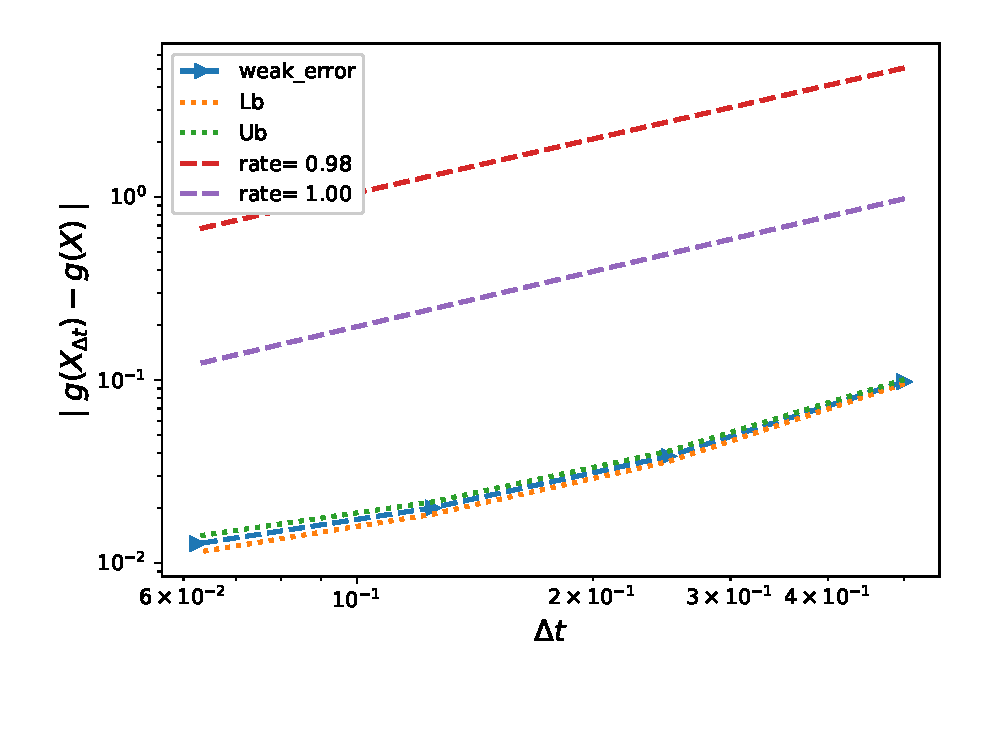
\includegraphics[width=0.4\linewidth]{./figures/binary_weak_error/without_richardson/weak_convergence_order_binary_option_relative_M_10_4}
%		\caption{}
%		\label{fig:sub3}
%	\end{subfigure}%
%	\begin{subfigure}{.35\textwidth}
%		\centering
%		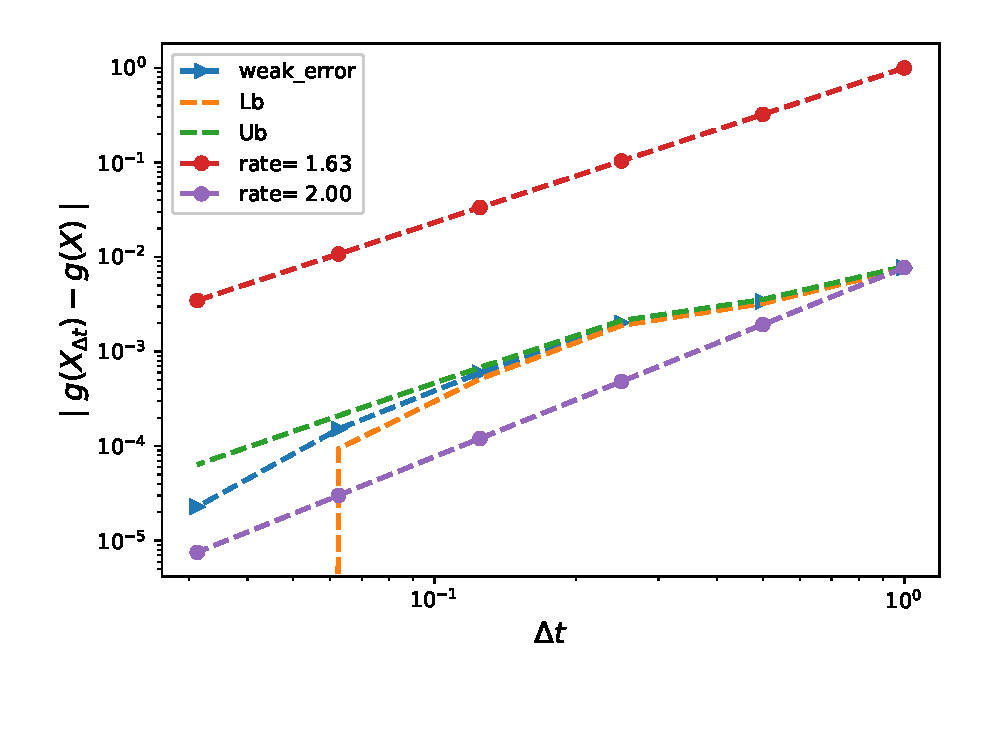
\includegraphics[width=1\linewidth]{./figures/binary_weak_error/with_richardson/weak_convergence_order_binary_richardson_relative_M_5_10_6}
%		\caption{}
%		\label{fig:sub4}
%	\end{subfigure}
	
	\caption{The convergence of the relative weak error  $\mathcal{E}_B(N)$ defined in \ref{eq:total_error}, using MC with $M=10^4$ samples  for the binary option example. The upper and lower bounds are $95\%$ confidence intervals.}
	\label{fig:Weak_rate_binary}
\end{figure}

\FloatBarrier


%\begin{figure}[h!]
%	\centering
%	\begin{subfigure}{.4\textwidth}
%		\centering
%		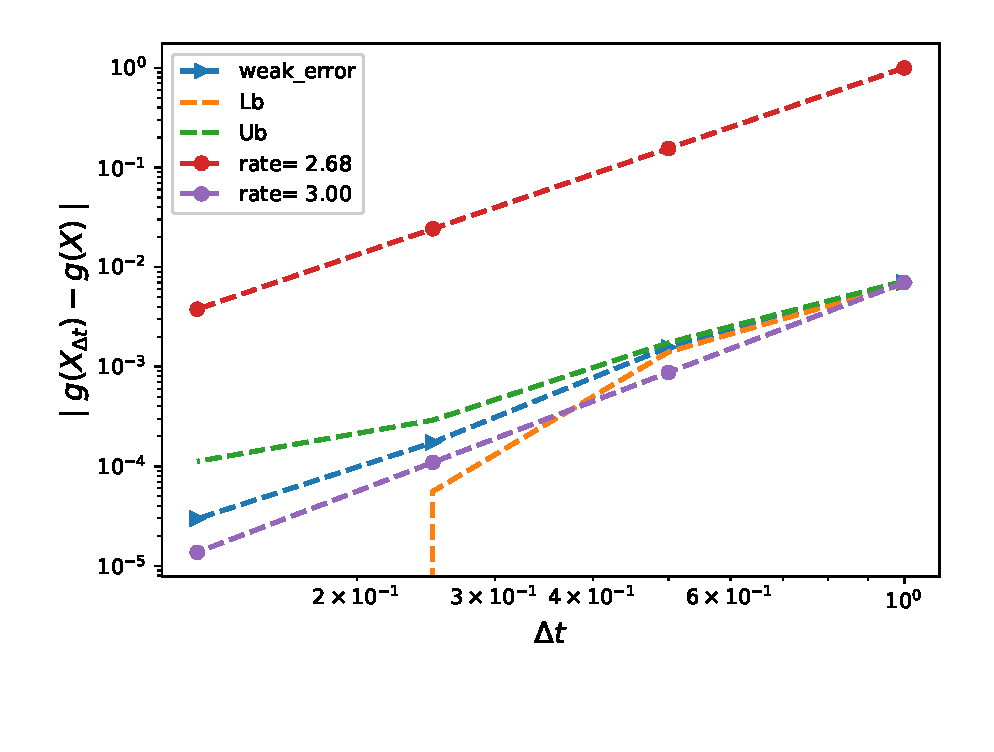
\includegraphics[width=1\linewidth]{./figures/binary_weak_error/with_richardson/weak_convergence_order_binary_richardson_level2_relative_M_5_10_6}
%		\caption{}
%		\label{fig:sub3}
%	\end{subfigure}%
%	\begin{subfigure}{.4\textwidth}
%		\centering
%		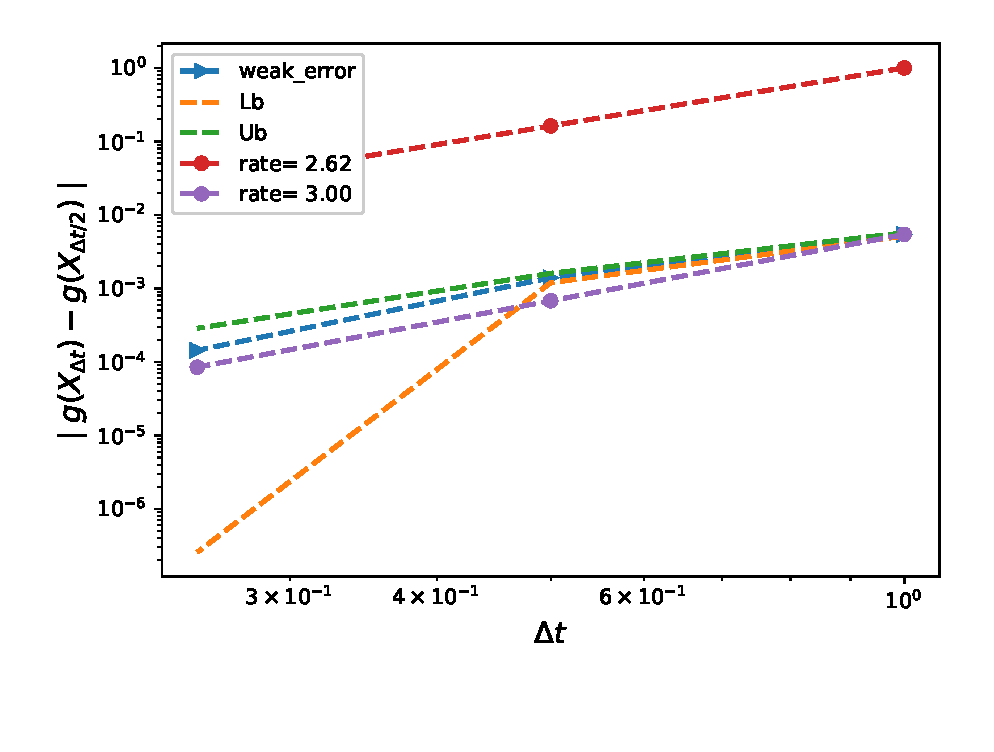
\includegraphics[width=1\linewidth]{./figures/binary_weak_error/with_richardson/weak_convergence_order_differences_binary_richardson_level2_relative_M_5_10_6}
%		\caption{}
%		\label{fig:sub4}
%	\end{subfigure}
%	
%	\caption{The rate of convergence of the weak error for the binary option, with Richardson extraploation (level $2$), using MC with $M=5.10^6$: a) $\abs{\frac{1}{3}\expt{8 g(X_{\Delta t/4}) -6g(X_{\Delta t/2}) +g(X_{\Delta t})}-g(X)}$  b) $\abs{\frac{1}{3}\expt{-8 g(X_{\Delta t/8}) +14g(X_{\Delta t/4})-7 (X_{\Delta t/2}) +g(X_{\Delta t})}}$ }
%	\label{fig:fig:Weak_rate_binary_with_rich_level2}
%\end{figure}
%
%\subsubsection{Comparing relative errors}\label{sec:Comparing relative errors, binary}


%\FloatBarrier
%\begin{table}[h!]
%	\centering
%	\begin{tabular}{l*{6}{c}r}
%		Method \textbackslash  Steps            & $2$ & $4$ & $8$ & $16$ &   \\
%		\hline
%		MISC ($TOL_{\text{MISC}}=5.10^{-1}$)  & $0.4620$ & $0.4404$ & $0.4299$ & $0.4250$  \\
%		MISC ($TOL_{\text{MISC}}=10^{-1}$)  & $0.4620$ & $0.4404$ & $0.4301$ & $0.4250$  \\
%		MISC ($TOL_{\text{MISC}}=5.10^{-2}$)  & $0.4620$ & $0.4403$ & $0.4300$ & $0.4250$  \\
%		MISC ($TOL_{\text{MISC}}=10^{-2}$)  & $0.4620$ & $0.4406$ &  $0.4300$ & $0.4250$  \\
%		MISC ($TOL_{\text{MISC}}=10^{-3}$)  & $0.4620$ & $0.4406$ & $0.4301$  & $0.4254$  \\
%%		MISC ($TOL_{\text{MISC}}=10^{-4}$)  & $0.4620$ & $0.4406$ &  $0.4301$ & $-$  \\
%		\hline
%	%	MC method ($M=10^{5}$)   & $-$ & $-$  & $-$ & $-$ \\		
%		MC method ($M=10^{4}$)   & $  0.4620$ & $    0.4369
%		$  & $      0.4292$ & $  
%		0.4261$ \\	
%		\hline
%	\end{tabular}
%	\caption{Binary option price of the different methods for different number of time steps, without Richardson extrapolation.}
%	\label{table: Binary option price of the different methods for different number of time steps, without Richardson extrapolation.}
%\end{table}

%\begin{table}[h!]
%	\centering
%	\begin{tabular}{l*{6}{c}r}
%		Method \textbackslash  Steps            & $2$ & $4$ & $8$ & $16$  \\
%		\hline
%		MC Bias $(M=10^{4})$  & 	$ \underset{(    
%			0.0412)}{\mathbf{0.0980}}$  & $\underset{( 0.0162)}{\mathbf{ 0.0384
%		}}$  & $\underset{(    0.0085
%	)}{\mathbf{0.0201}}$ & $\underset{(   0.0053)}{\mathbf{   0.0127}}$\\ 
%		
%		MC Statistical error $(M=10^{4})$  &  $\underset{( 5.0e-04)} {\mathbf{1.2e-03}}$  & $\underset{( 5.0e-04)} {\mathbf{1.2e-03}}$ & $\underset{(3.4e-04)} {\mathbf{8.0e-04}}$ & $\underset{( 2.7e-04)} {\mathbf{6.5e-04}}$	\\
%%			MC: Statistical error ($M=10^6$)  &  $\underset{( 5.0e-04)} {\mathbf{1.2e-03}}$  & $\underset{( 5.0e-04)} {\mathbf{1.2e-03}}$ & $\underset{( 5.0e-04)} {\mathbf{1.2e-03}}$ & $\underset{( 5.0e-04)} {\mathbf{1.2e-03}}$	\\
%		\hline
%	\end{tabular}
%	\caption{Bias and statistical errors of MC  for computing binary option price  for different number of time steps, without Richardson extrapolation. The numbers between parentheses are the corresponding absolute errors.}
%	\label{Bias and Statistical errors of MC  for computing Binary option price  for different number of time steps, without Richardson extrapolation. The numbers between parentheses are the corresponding absolute errors.}
%\end{table}
%
%\FloatBarrier
%
%
%
%
%\begin{table}[h!]
%	\centering
%	\begin{tabular}{l*{6}{c}r}
%		Method \textbackslash  Steps            & $2$ & $4$ & $8$ & $16$  \\
%		\hline
%		MISC ($TOL_{\text{MISC}}=5.10^{-1}$)  & $\underset{(2.4e-05)}{\mathbf{\red{1.0e-05}}}$ & $\underset{(0.0035)}{\mathbf{0.0083}}$  & $\underset{(0.0007)}{\mathbf{ 0.0017}}$ &$\underset{(0.0011)}{\mathbf{0.0026}}$ \\
%		MISC ($TOL_{\text{MISC}}=10^{-1}$)   & $\underset{(2.4e-05)}{\mathbf{1.0e-05}}$ & $\underset{(0.0035)}{\mathbf{0.0083}}$ & $\underset{(0.0009)}{\mathbf{\red{0.0021}}}$ & $\underset{(0.0011)}{\mathbf{
%				0.0026}}$ \\
%		MISC ($TOL_{\text{MISC}}=5.10^{-2}$)  & $\underset{(2.4e-05)}{\mathbf{1.0e-05}}$& $\underset{(0.0034)}{\mathbf{0.0081}}$ & $\underset{(0.0008)}{\mathbf{ 0.0019}}$& $\underset{(0.0011)}{\mathbf{
%				0.0026}}$ \\
%		MISC ($TOL_{\text{MISC}}=10^{-2}$)  & $\underset{(2.4e-05)}{\mathbf{1.0e-05}}$ & $\underset{(0.0037)}{\mathbf{\red{0.0088}}}$ & $\underset{(0.0008)}{\mathbf{ 0.0019}}$ & $\underset{(0.0011)}{\mathbf{
%				0.0026}}$ \\
%		MISC ($TOL_{\text{MISC}}=10^{-3}$)  & $\underset{(2.4e-05)}{\mathbf{1.0e-05}}$ & $\underset{(0.0037)}{\mathbf{0.0088}}$& $\underset{(0.0009)}{\mathbf{0.0021}}$& $\underset{(0.0007)}{\mathbf{\red{ 0.0017}}}$ \\
%%			MISC ($TOL_{\text{MISC}}=10^{-4}$)  & $\underset{(2.4e-05)}{\mathbf{1.0e-05}}$ & $\underset{(0.0037)}{\mathbf{0.0088}}$& $\underset{(0.0009)}{\mathbf{0.0021}}$& $\underset{(-)}{\mathbf{ -}}$ \\
%		\hline
%	\end{tabular}
%	\caption{Quadrature error of MISC,  with different tolerances, to compute binary option price for different number of time steps, without Richardson extrapolation. The numbers between parentheses are the corresponding absolute errors. The values marked in red correspond to stable quadrature errors for MISC, and will be used for complexity comparison against MC.}
%	\label{Quadrature error of MISC to compute Binary option price of the different tolerances for different number of time steps, without Richardson extrapolation. The numbers between parentheses are the corresponding absolute errors.}
%\end{table}

%\FloatBarrier
%	\begin{figure}[h!]
%	\centering
%	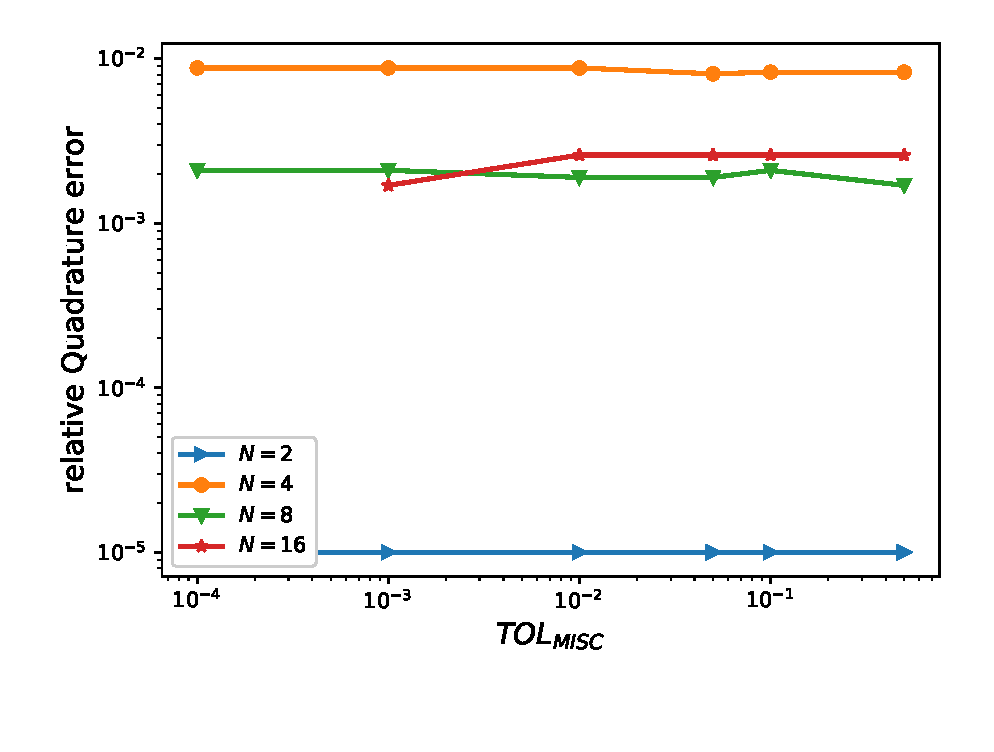
\includegraphics[width=0.4\linewidth]{./figures/Binary_MISC_quadrature_error/relative_quad_error_wrt_MISC_TOL_non_rich}
%	
%	
%	\caption{Relative quadrature error of MISC, with different tolerances, to compute binary option price for different number of time steps, without Richardson extrapolation.}
%	\label{fig:Quadrature_error_non_rich_binary}
%\end{figure}
\FloatBarrier

\begin{table}[h!]
	\centering
	\begin{tabular}{l*{6}{c}r}
		\toprule[1.5pt]
	Method & & Steps  &     \\
	\hline
	        & $4$ & $8$ & $16$  \\
		\hline
%		($TOL_{\text{MISC}}=5.10^{-1}$) 
		MISC   & $\underset{(0.04,0.01 )}{\mathbf{0.05}}$ & $\underset{(0.02,0.002)}{\mathbf{ 0.02}}$ & $\underset{(0.01,0.002)}{\mathbf{0.01}}$  \\
%		MISC ($TOL_{\text{MISC}}=10^{-1}$) & $\underset{(0.04,0.01 )}{\mathbf{0.05}}$ & $\underset{(0.02,0.002)}{\mathbf{\red{0.02}}}$ & $\underset{(0.013,0.002)}{\mathbf{0.015}}$   \\
%		MISC ($TOL_{\text{MISC}}=5.10^{-2}$)  & $\underset{(0.04, 0.01)}{\mathbf{0.05}}$ & $\underset{(0.02,0.002)}{\mathbf{0.02}}$ & $\underset{(0.013,0.002)}{\mathbf{0.015}}$  \\
%		MISC ($TOL_{\text{MISC}}=10^{-2}$)  & $\underset{(0.04, 0.01)}{\mathbf{\red{ 0.05}}}$ & $\underset{(0.02,0.002)}{\mathbf{ 0.02}}$ & $\underset{(0.013,0.002)}{\mathbf{0.015}}$    \\
%		MISC ($TOL_{\text{MISC}}=10^{-3}$)   & $\underset{(0.04, 0.01)}{\mathbf{ 0.05}}$  & $\underset{(0.02,0.002)}{\mathbf{ 0.02}}$  & $\underset{(0.013,0.002)}{\mathbf{\red{0.015}}}$\\
		\hline
		MC+root finding   &   $\underset{(0.04,0.04 )}{\mathbf{0.08}}$ & $\underset{(0.02,0.02)}{\mathbf{0.04}}$ & $\underset{(0.01,0.01)}{\mathbf{0.02}}$  \\	
			M(\# MC samples)   & $ 10^1$  & $4 \times 10^1$  & $  10^2$ \\	
		\hline
			MC     & $\underset{(0.05,0.05)}{\mathbf{0.1}}$ & $\underset{(0.025,0.025 )}{\mathbf{0.05}}$ & $\underset{(0.01,0.01 )}{\mathbf{0.02}}$  \\	
			M(\# MC samples)   & $ 10^3$  & $8 \times 10^3$  & $ 5 \times 10^4$ \\	
			\bottomrule[1.25pt]
	\end{tabular}
	\caption{Total relative error of MISC, with different tolerances, and MC to compute binary option price for different number of time steps, without Richardson extrapolation. The values between parentheses correspond to the different errors contributing to the total relative error: for MISC we report the bias and quadrature errors and for MC we report the bias and the statistical errors. The number of MC samples,$ M$, is chosen to satisfy \eqref{optimal_number_samples}.}
	\label{Total error of MISC and MC to compute Binary option price of the different tolerances for different number of time steps, without Richardson extrapolation. The numbers between parentheses are the corresponding absolute errors.}
\end{table}

\FloatBarrier

\begin{table}[h!]
	\centering
	\begin{tabular}{l*{6}{c}r}
		\toprule[1.5pt]
	Method & & Steps  &     \\
	\hline
		         & $4$ & $8$ & $16$ &   \\
		\hline
%		 ($TOL_{\text{MISC}}=5.10^{-1}$)
		MISC   & $0.8$ & $2$ & $9$  \\
%		MISC ($TOL_{\text{MISC}}=10^{-1}$)   & $0.8$ & $\red{9}$ & $49$  \\
%		MISC ($TOL_{\text{MISC}}=5.10^{-2}$)    & $1.3$ & $12$ & $59$  \\
%		MISC ($TOL_{\text{MISC}}=10^{-2}$)   & $\red{2}$ & $14$ & $63$  \\
%		MISC ($TOL_{\text{MISC}}=10^{-3}$)    & $2$ & $34$ & $\red{1090}$  \\
%    	MISC ($TOL_{\text{MISC}}=10^{-4}$)   & $0.3$ & $16$ & $193$ & $-$  \\
		\hline
		MC+root finding     & $0.2$ & $1$ & $9$  \\
		\hline 
		MC     & $0.3$ & $3$ & $29$  \\
%		\hline
%		Ratio of	$\text{(MC+root finding)}/\text{(MISC)}$  & $\red{4.5}$ & $\red{11}$ & $\red{0.13}$  \\
%			Ratio of	$(\text{MC})/(\text{MISC})$ &  $\red{3.5}$ & $\red{11}$ & $\red{0.14}$  \\
				\bottomrule[1.25pt]
	\end{tabular}
	\caption{Comparison of the computational time of  MC and MISC, used to compute binary option price  for different number of time steps, without Richardson extrapolation. The average computational time of MC is computed over $10$ runs.}
	\label{Comparsion of the computational time of  MC and MISC, used to compute Binary option price  for different number of time steps, without Richardson extrapolation}
\end{table}



\FloatBarrier
\begin{figure}[h!]
\centering
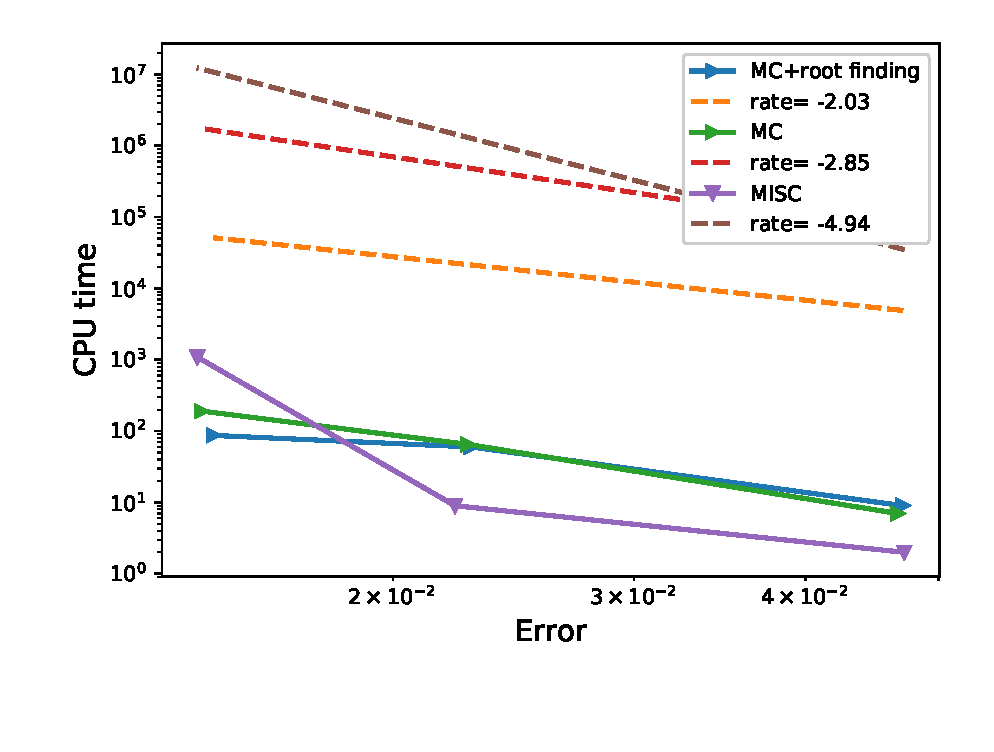
\includegraphics[width=0.4\linewidth]{./figures/Binary_Complexity_rates/error_vs_time}
	\caption{Computational work comparison for MISC and MC methods, for the case of binary  option. This plot shows that to achieve a relative error below $1\%$, MISC outperforms  MC method in terms of computational time}
	\label{fig:Complexity plot for MC and MISC , Binary, Non rich}
\end{figure}

%\FloatBarrier
%
%\subsubsection*{With Richardson extrapolation (level $1$)}
%
%
%%\FloatBarrier
%%
%%\begin{table}[h!]
%%	\centering
%%	\begin{tabular}{l*{6}{c}r}
%%		Method \textbackslash  Steps            & $1-2$ & $2-4$ & $4-8$ & $8-16$ &   \\
%%		\hline
%%		MISC ($TOL_{\text{MISC}}=5.10^{-1}$)  & $0.4239$ & $0.4188$ & $0.4191$ & $0.4200$  \\
%%		MISC ($TOL_{\text{MISC}}=10^{-1}$)  &$0.4239$ & $0.4188$ &$0.4191$ & $0.4199$  \\
%%		MISC ($TOL_{\text{MISC}}=5.10^{-2}$) & $0.4239$ & $0.4188$ & $0.4190$ & $0.4199$  \\
%%		MISC ($TOL_{\text{MISC}}=10^{-2}$) &$0.4239$ & $0.4192$ & $0.4194$ & $0.4199$  \\
%%%		MISC ($TOL_{\text{MISC}}=10^{-3}$) & $0.4239$ & $0.4192$ & $0.4199$ & $0.4205$  \\
%%%			MISC ($TOL_{\text{MISC}}=10^{-4}$) & $0.4239$ & $0.4193$ & $0.4199$ & $-$  \\
%%		\hline
%%		MC method ($M=5.10^{6}$)   & $ 0.4240$ & $
%%		0.4224$ & $    0.4216$ & $  0.4210$  \\
%%		\hline
%%	\end{tabular}
%%	\caption{Binary option price of the different methods for different number of time steps, with Richardson extrapolation (level $1$).}
%%	\label{table: Binary option price of the different methods for different number of time steps, with Richardson extrapolation (level1).}
%%\end{table}
%%
%%\FloatBarrier
%%\begin{table}[h!]
%%	\centering
%%	\begin{tabular}{l*{6}{c}r}
%%		Method \textbackslash  Steps            & $1-2$ & $2-4$ & $4-8$ & $8-16$  \\
%%		\hline
%%	MC Bias  ($M=5.10^{6}$)&$ \underset{(0.0032)}{\mathbf{0.0077}}$    & $\underset{(    0.0016
%%		)}{\mathbf{0.0039}}$  & $\underset{(0.0008)}{\mathbf{0.0020}}$  & $\underset{(0.0003)}{\mathbf{0.0006}}$\\
%%		MC Statistical error   ($M=5.10^{6}$)   & 	$ \underset{( 4.6e-05  )}{\mathbf{1.1e-04}}$  & $\underset{(3.5e-05)}{\mathbf{ 8.4e-05
%%	}}$  & $\underset{(2.5e-05)}{\mathbf{6.0e-05}}$ & $\underset{(   1.8e-05 )}{\mathbf{  4.2e-05 }}$\\ 
%%		
%%%		MC+root finding: Statistical error ($M=10^3$)     & 	$ \underset{( 3.5e-03  )}{\mathbf{8.3e-03}}$  & $\underset{(2.8e-03)}{\mathbf{ 6.6e-03
%%%		}}$  & $\underset{(1.8e-03)}{\mathbf{4.3e-03}}$ & $\underset{(  1.2e-03 )}{\mathbf{  2.9e-03 }}$\\ 
%%%		
%%		\hline
%%	\end{tabular}
%%	\caption{Bias and statistical errors of MC  for computing binary option price  for different number of time steps, with Richardson extrapolation (level $1$). The numbers between parentheses are the corresponding absolute errors.}
%%	\label{Bias and Statistical errors of MC  for computing Binary option price  for different number of time steps, with Richardson extrapolation (level $1$). The numbers between parentheses are the corresponding absolute errors.}
%%\end{table}
%
%%\FloatBarrier
%%
%%
%%
%%\begin{table}[h!]
%%	\centering
%%	\begin{tabular}{l*{6}{c}r}
%%		Method \textbackslash  Steps            & $1-2$ & $2-4$ & $4-8$ & $8-16$  \\
%%		\hline
%%		MISC ($TOL_{\text{MISC}}=5.10^{-1}$)  & $\underset{(   1.0e-04)}{\mathbf{ \red{2.4e-04}}}$ & $\underset{(3.6e-03)}{\mathbf{8.6e-03}}$  & $\underset{(2.5e-03)}{\mathbf{5.9e-03}}$ &$\underset{(1.0e-03)}{\mathbf{2.4e-03}}$ \\
%%		MISC ($TOL_{\text{MISC}}=10^{-1}$)   & $\underset{(   1.0e-04)}{\mathbf{ 2.4e-04}}$ & $\underset{(3.6e-03)}{\mathbf{8.6e-03}}$  & $\underset{(2.5e-03)}{\mathbf{5.9e-03}}$ &$\underset{(   1.1e-04)}{\mathbf{ \red{2.6e-03}}}$ \\
%%		MISC ($TOL_{\text{MISC}}=5.10^{-2}$)  & $\underset{(   1.0e-04)}{\mathbf{ 2.4e-04}}$ & $\underset{(3.6e-03)}{\mathbf{8.6e-03}}$ & $\underset{(2.6e-03)}{\mathbf{6.2e-03}}$ &$\underset{(   1.1e-04)}{\mathbf{ 2.6e-03}}$ \\
%%		MISC ($TOL_{\text{MISC}}=10^{-2}$)  & $\underset{(   1.0e-04)}{\mathbf{ 2.4e-04}}$ & $\underset{(3.2e-03)}{\mathbf{\red{7.6e-03}}}$  & $\underset{(2.2e-03)}{\mathbf{\red{5.2e-03}}}$ &$\underset{(   1.1e-04)}{\mathbf{ 2.6e-03}}$\\
%%%		MISC ($TOL_{\text{MISC}}=10^{-3}$)  & $\underset{(   1.0e-04)}{\mathbf{ 2.4e-04}}$ & $\underset{(3.2e-03)}{\mathbf{7.6e-03}}$  & $\underset{(1.7e-03)}{\mathbf{4.0e-03}}$ &$\underset{(   5.e-04)}{\mathbf{1.2e-03}}$ \\
%%%	MISC ($TOL_{\text{MISC}}=10^{-4}$)  & $\underset{(   1.0e-04)}{\mathbf{ 2.4e-04}}$ & $\underset{(3.1e-03)}{\mathbf{7.4e-03}}$  & $\underset{(1.7e-03)}{\mathbf{4.0e-03}}$ &$\underset{()}{\mathbf{}}$ \\
%%		\hline
%%	\end{tabular}
%%	\caption{Quadrature error of MISC, with different tolerances,  to compute binary option price for different number of time steps, with Richardson extrapolation (level $1$). The numbers between parentheses are the corresponding absolute errors. The values marked in red correspond to stable quadrature errors for MISC, and will be used for complexity comparison against MC.}
%%	\label{Quadrature error of MISC to compute Binary option price of the different tolerances for different number of time steps, with Richardson extrapolation (level $1$). The numbers between parentheses are the corresponding absolute errors.}
%%\end{table}
%%
%%
%%\FloatBarrier
%%	\begin{figure}[h!]
%%	\centering
%%	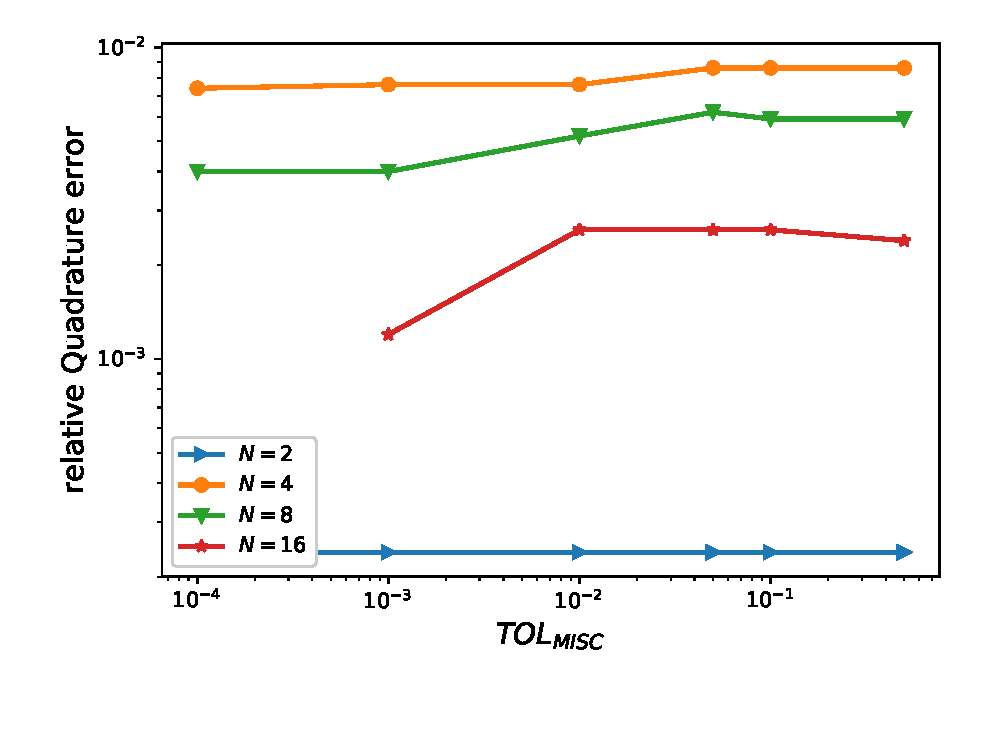
\includegraphics[width=0.4\linewidth]{./figures/Binary_MISC_quadrature_error/relative_quad_error_wrt_MISC_TOL_with_rich}
%%	
%%	
%%	\caption{Relative quadrature error of MISC, with different tolerances, to compute binary option price of the different tolerances for different number of time steps, with Richardson extrapolation.}
%%	\label{fig:Quadrature_error_with_rich_binary}
%%\end{figure}
%
%\FloatBarrier
%
%\begin{table}[h!]
%	\centering
%	\begin{tabular}{l*{6}{c}r}
%		\toprule[1.5pt]
%	Method & & Steps  &     \\
%	\hline
%		        & $2-4$ & $4-8$ & $8-16$  \\
%		\hline
%		MISC ($TOL_{\text{MISC}}=5.10^{-1}$)  & $\underset{(0.004,0.009)}{\mathbf{0.013}}$ & $\underset{(0.002,0.006)}{\mathbf{0.008}}$ & $\underset{(0.0006,0.0016)}{\mathbf{0.002}}$  \\
%%		MISC ($TOL_{\text{MISC}}=10^{-1}$)  &    $\underset{(0.004,0.009)}{\mathbf{0.013}}$ & $\underset{(0.002,0.006)}{\mathbf{0.008}}$ & $\underset{(0.0006,0.0026)}{\mathbf{\red{0.003}}}$  \\
%%		MISC ($TOL_{\text{MISC}}=5.10^{-2}$) & $\underset{(0.004,0.009)}{\mathbf{0.013}}$ & $\underset{(0.002,0.006)}{\mathbf{0.008}}$ & $\underset{(0.0006,0.0026)}{\mathbf{0.003}}$  \\
%%		MISC ($TOL_{\text{MISC}}=10^{-2}$)   & $\underset{(0.004,0.008)}{\mathbf{\red{0.012}}}$ & $\underset{(0.002,0.005)}{\mathbf{\red{0.007}}}$ & $\underset{(0.0006,0.0026)}{\mathbf{0.003}}$  \\
%%		MISC ($TOL_{\text{MISC}}=10^{-3}$) &   $\mathbf{0.0079}$ & $\mathbf{0.0115}$ & $\mathbf{0.0060}$ & $\mathbf{0.0018}$  \\
%%
%%	MISC ($TOL_{\text{MISC}}=10^{-4}$) &   $\mathbf{0.0079}$ & $\mathbf{0.0113}$ & $\mathbf{0.0060}$ & $\mathbf{-}$  \\
%		\hline
%		MC+root finding   & $\underset{(0.004,)}{\mathbf{\red{0.008}}}$ & $\underset{(0.002,)}{\mathbf{\red{0.004}}}$ & $\underset{(0.0006,)}{\mathbf{\red{0.001}}}$  \\	
%			MC     & $\mathbf{\red{0.0116}}$ & $\mathbf{\red{0.0073}}$ & $\mathbf{\red{0.0029}}$  \\	
%			\bottomrule[1.25pt]
%	\end{tabular}
%	\caption{Total relative error of MISC, with different tolerances, and MC to compute binary option price for different number of time steps, with Richardson extrapolation (level $1$).  The values marked in red, for MISC method, correspond to the total relative errors associated with  stable quadrature errors for MISC, and will be used for complexity comparison against MC.}
%	\label{Total error of MISC and MC to compute Binary option price of the different tolerances for different number of time steps, with Richardson extrapolation (level $1$). The numbers between parentheses are the corresponding absolute errors.}
%\end{table}
%
%
%
%\FloatBarrier
%
%
%\begin{table}[h!]
%	\centering
%	\begin{tabular}{l*{6}{c}r}
%		\toprule[1.5pt]
%	Method & & Steps  &     \\
%	\hline
%		   & $2-4$ & $4-8$ & $8-16$ &   \\
%		\hline
%		MISC ($TOL_{\text{MISC}}=5.10^{-1}$) & $1$ & $4$ & $9$  \\
%%		MISC ($TOL_{\text{MISC}}=10^{-1}$) & $1$ & $8$ & $\red{42}$  \\
%%		MISC ($TOL_{\text{MISC}}=5.10^{-2}$)  & $1$ & $10$ & $72$  \\
%%		MISC ($TOL_{\text{MISC}}=10^{-2}$)   & $\red{4}$ & $\red{15}$ & $78$  \\
%%		MISC ($TOL_{\text{MISC}}=10^{-3}$)   &$0.3$ & $4$ & $100$ & $2253$  \\
%%			MISC ($TOL_{\text{MISC}}=10^{-4}$)   &$0.3$ & $68$ & $392$ & $$  \\
%		\hline
%		MC+root finding method      & $\red{48}$ & $\red{62}$ & $\red{122 }$  \\
%			MC    & $\red{12}$ & $\red{23}$ & $\red{147}$  \\
%%		\hline
%%			Ratio of	$\text{(MC+root finding)}/\text{(MISC)}$  & $\red{12}$ & $\red{4.1}$ & $\red{2.9}$  \\
%%		Ratio of	$(\text{MC})/(\text{MISC})$ & $\red{3}$ & $\red{1.5}$ & $\red{3.5}$  \\
%		\bottomrule[1.25pt]
%	\end{tabular}
%	\caption{Comparison of the computational time of  MC and MISC, used to compute binary option price  for different number of time steps, with Richardson extrapolation (level $1$). The average computational time of MC is computed over $10$ runs.}
%	\label{Comparsion of the computational time of  MC and MISC, used to compute Binary option price  for different number of time steps, with Richardson extrapolation (level $1$)}
%\end{table}
%
%\FloatBarrier
%	\begin{figure}[h!]
%\centering
%\includegraphics[width=0.4\linewidth]{./figures/Binary_Complexity_rates/error_vs_time_rich}
%
%\caption{Complexity plot for MC and MISC for the case with Richardson extrapolation.}
%\label{fig:Complexity plot for MC and MISC , Binary, with rich}
%\end{figure}
%
%
%
%
%
%
%\FloatBarrier
%
%\begin{figure}[h!]
%\centering
%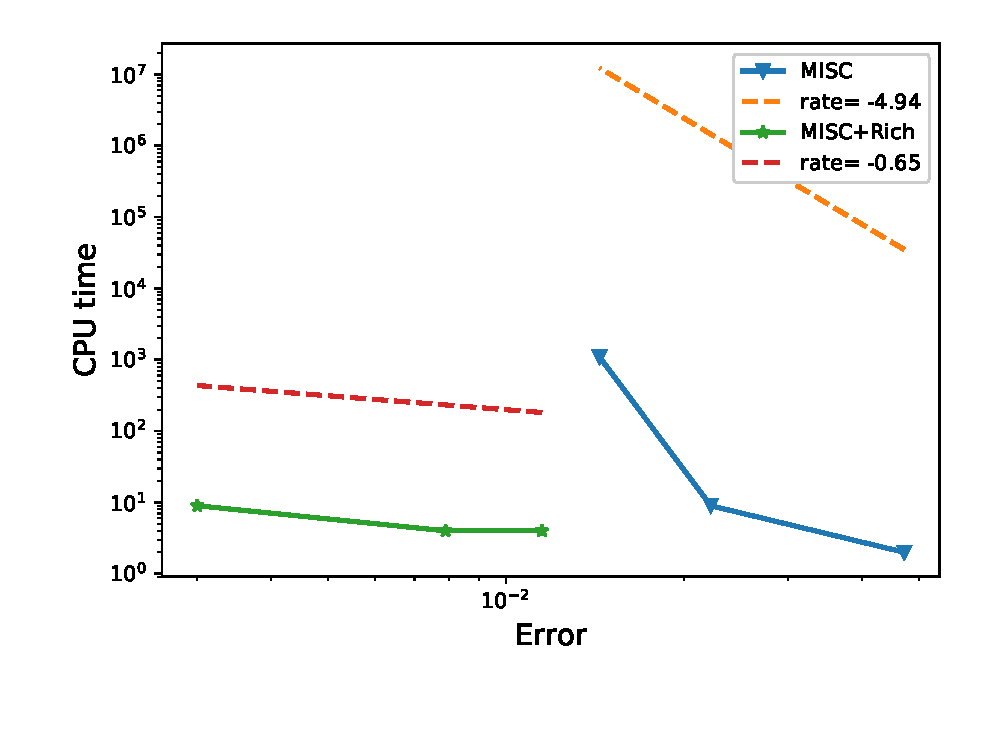
\includegraphics[width=0.4\linewidth]{./figures/Binary_Complexity_rates/error_vs_time_comparison}
%
%\caption{Complexity plot for MISC without and with Richardson extrapolation, for the binary option.}
%\label{fig:Complexity plot for MC and MISC , Binary, comparison}
%\end{figure}
%
%\FloatBarrier
%


%In the following, we compare the  relative errors for the binary option example under Black-Scholes model (see Tables (\ref{Relative error of the binary option price of the different tolerances for different number of time steps.}, \ref{Relative error of Call option price of the different tolerances for different number of time steps, using Richardson extrapolation (level $1$)})). We report the results for $2$ scenarios: i) Without using Richardson extrapolation, ii) Using level $1$ Richardson extrapoaltion.  You may see appendix \ref{appendix:Call prices for different methods_binary} for the values of binary option prices.
%
%Given the normalized bias computed by MC method (See Section \ref{sec:Weak error plots_binary}) (reported as bold values in the tables), we report in red in each table the smallest tolerance that MISC required to get below that relative bias (I do not put values for smaller tolerances, once the required bias is reached).
%
%From the tables (\ref{Relative error of the binary option price of the different tolerances for different number of time steps.}, \ref{Relative error of Call option price of the different tolerances for different number of time steps, using Richardson extrapolation (level $1$)})), we may observe that to get a relative error below $1\%$, we need around $16$ time steps for the case without Richardson extrapolation compared to only using $1$ time step in the coarse level for the case of level $1$ Richardson extraplation. 



%\begin{table}[h!]
%	\centering
%	\begin{tabular}{l*{5}{c}r}
%		Method \textbackslash  Steps    &$1-2$        & $2-4$ & $4-8$ & $8-16$  \\
%		\hline
%		MISC ($TOL_{\text{MISC}}=5.10^{-1}$)  &$\red{0.0076}$ & $0.0045$ & $0.0031$ & $0.0017$  \\
%		MISC ($TOL_{\text{MISC}}=10^{-2}$)  &$-$ & $\red{0.0036}$ & $0.0031$ & $0.0014$  \\
%		MISC ($TOL_{\text{MISC}}=10^{-3}$) & $-$ & $-$ & $  \red{0.0021}$ & $\red{0.0005}$   \\
%		MC method ($M=5.10^{6}$)&$ \mathbf{0.0077}$    & $\mathbf{0.0039}$  & $\mathbf{0.0020}$  & $\mathbf{0.0006}$ \\
%		\hline
%	\end{tabular}
%	\caption{Relative error of the binary option price of the different tolerances for different number of time steps, using Richardson extrapolation (level $1$)}
%	\label{Relative error of binary option price of the different tolerances for different number of time steps, using Richardson extrapolation (level $1$)}
%\end{table}


\FloatBarrier
\subsubsection{Results for the single call option example}\label{sec:Results for the call option example}
In this case, the integrand $h(\mathbf{z}_{-1})$ is given by

\begin{align}\label{smoothed_integrand_call_opt_2}
h(\mathbf{z}_{-1})&= \int_{\rset}  \max \left(\Psi \circ \Phi(T;z_1,\mathbf{z}_{-1})-K,0\right) \frac{1}{\sqrt{2 \pi}} \operatorname{exp}(-z_1^2/2) dz_1 \PERIOD
\end{align}
We get the kink point by running Newton iteration with a precision of $10^{-10}$. We  decompose the total integration domain $\rset$  into sub-domains such that the integrand is smooth in the interior of  each sub-domain and such that the kink is located along the boundary of these areas. The total integral is then given as the sum of the separate integrals, \ie
\begin{align}
	h(\mathbf{z}_{-1}) &:=  \int_{\rset} \max \left(\Psi \circ \Phi(T;z_1,\mathbf{z}_{-1})-K,0\right) \frac{1}{\sqrt{2 \pi}} \operatorname{exp}(-z_1^2/2) dy \\ \nonumber
	&=\int_{-\infty}^{y^{\ast}} \max \left(\Psi \circ \Phi(T;z_1,\mathbf{z}_{-1})-K,0\right) \frac{1}{\sqrt{2 \pi}} \operatorname{exp}(-z_1^2/2) dz_1\\ \nonumber
	&+\int_{y^{\ast}}^{\infty} \max \left(\Psi \circ \Phi(T;z_1,\mathbf{z}_{-1})-K,0\right) \frac{1}{\sqrt{2 \pi}} \operatorname{exp}(-z_1^2/2) dz_1,
\end{align}
where we use Gauss-Laguerre quadrature with $\beta$ points to get each part.

The parameters that we used in our numerical experiments are: $T=1$, $\sigma=0.4$ and $S_0=K=100$. The exact value of this case is $15.85193755$.

Figure \ref{fig:Weak_rate_call_beta_32} shows the estimated   weak error  for the case without Richardson extrapolation, and we report the results for comparing MC and MISC in Tables \ref{Total error of MISC and MC to compute Call option price of the different tolerances for different number of time steps, without Richardson extrapolation. The numbers between parentheses are the corresponding absolute errors.} and \ref{Comparsion of the computational time of  MC and MISC, used to compute Call option price  for different number of time steps, without Richardson extrapolation}, and Figure \ref{fig:Complexity plot for MC and MISC , Call non rich}. Our numerical experiments show that MISC  requires approximately $5\%$ of the work of MC  to achieve a total relative error of around $0.9\%$.



%\subsubsection*{$\beta=10$}
%From figure \ref{fig:Weak_rate_call_without_rich}, we see that we get a weak error of order $\Delta t$. From figure \ref{fig:fig:Weak_rate_call_with_rich}, we observe that we get a weak error of order $\Delta t^2$ (if eliminate the  last point having a wide confidence interval point). From figure \ref{fig:Weak_rate_call_with_rich_level2}, we observe that we get an almost constant weak error, with that constant being the smallest cpmpared to without and with level $1$ Ricardson extrapolation. The upper and lower bounds are $95\%$ confidence interval.

%\begin{figure}[h!]
%	\centering
%	\begin{subfigure}{.35\textwidth}
%		\centering
%		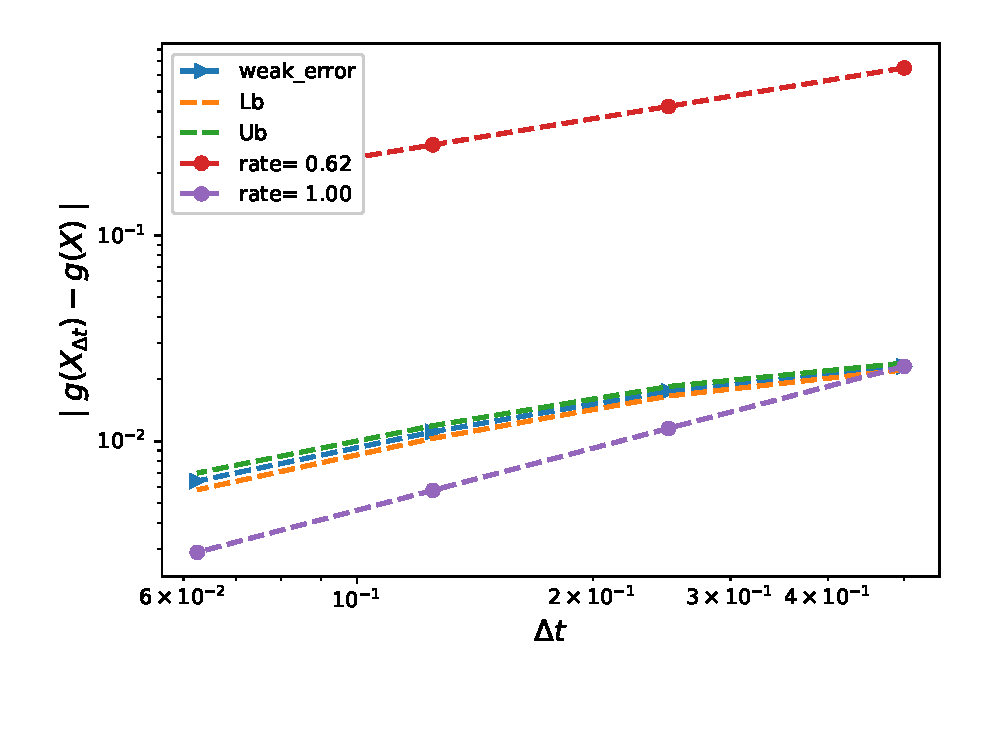
\includegraphics[width=1\linewidth]{./figures/weak_error_rates_call/Beta_10/without_richardson/weak_convergence_order_call_option_relative_M_10_5}
%		\caption{}
%		\label{fig:sub3}
%	\end{subfigure}%
%	\begin{subfigure}{.35\textwidth}
%		\centering
%		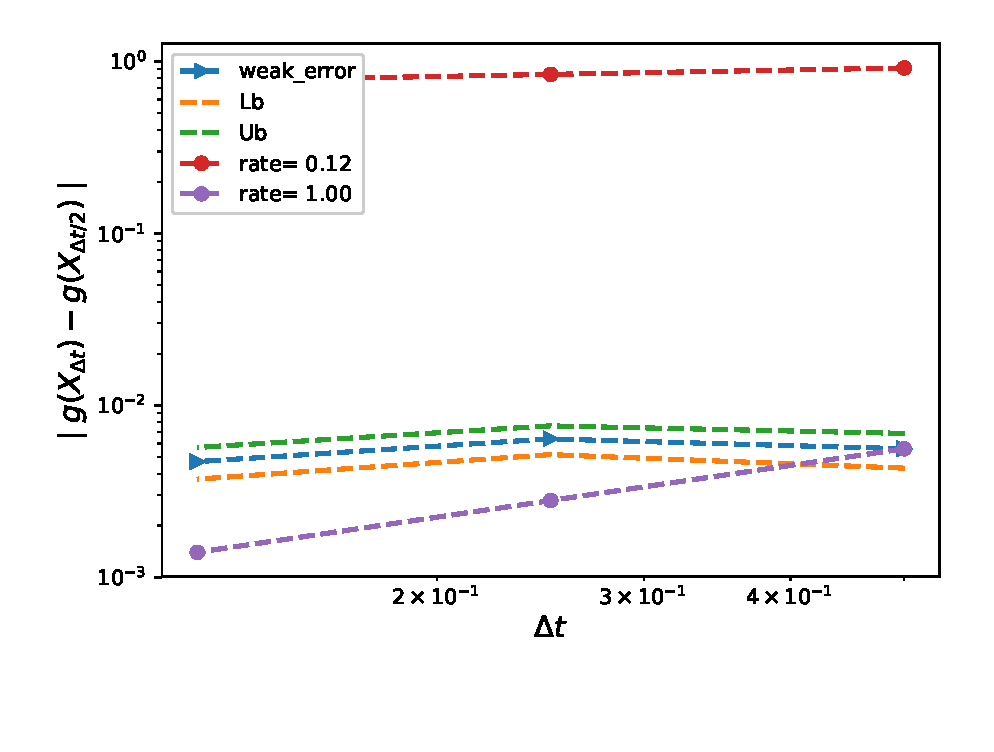
\includegraphics[width=1\linewidth]{./figures/weak_error_rates_call/Beta_10/without_richardson/weak_convergence_order_differences_call_option_relative_M_10_5}
%		\caption{}
%		\label{fig:sub4}
%	\end{subfigure}
%	
%	\caption{The rate of convergence of the weak error for the call option, without Richardson extraploation, using MC with $M=10^5$: a) $\abs{\expt{g(X_{\Delta t})}-g(X)}$  b) $\abs{\expt{g(X_{\Delta t})-g(X_{\Delta t/2})}}$ }
%	\label{fig:Weak_rate_call_without_rich}
%\end{figure}
%\begin{figure}[h!]
%	\centering
%	\begin{subfigure}{.35\textwidth}
%		\centering
%		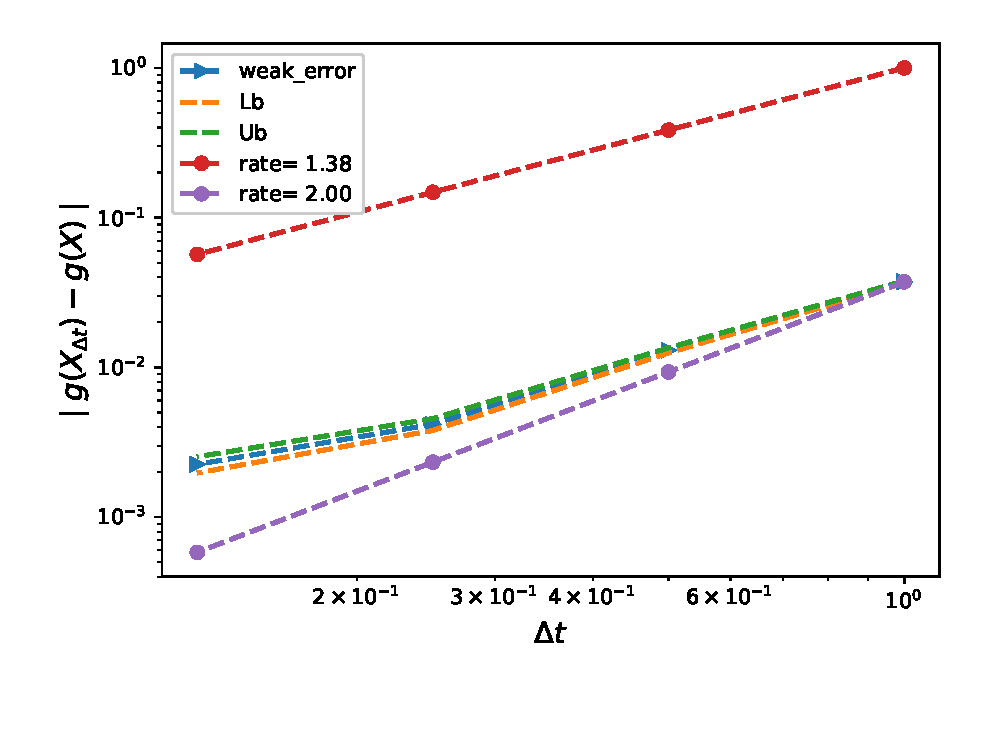
\includegraphics[width=1\linewidth]{./figures/weak_error_rates_call/Beta_10/with_richardson/weak_convergence_order_call_richardson_relative_M_10_6}
%		\caption{}
%		\label{fig:sub3}
%	\end{subfigure}%
%	\begin{subfigure}{.35\textwidth}
%		\centering
%		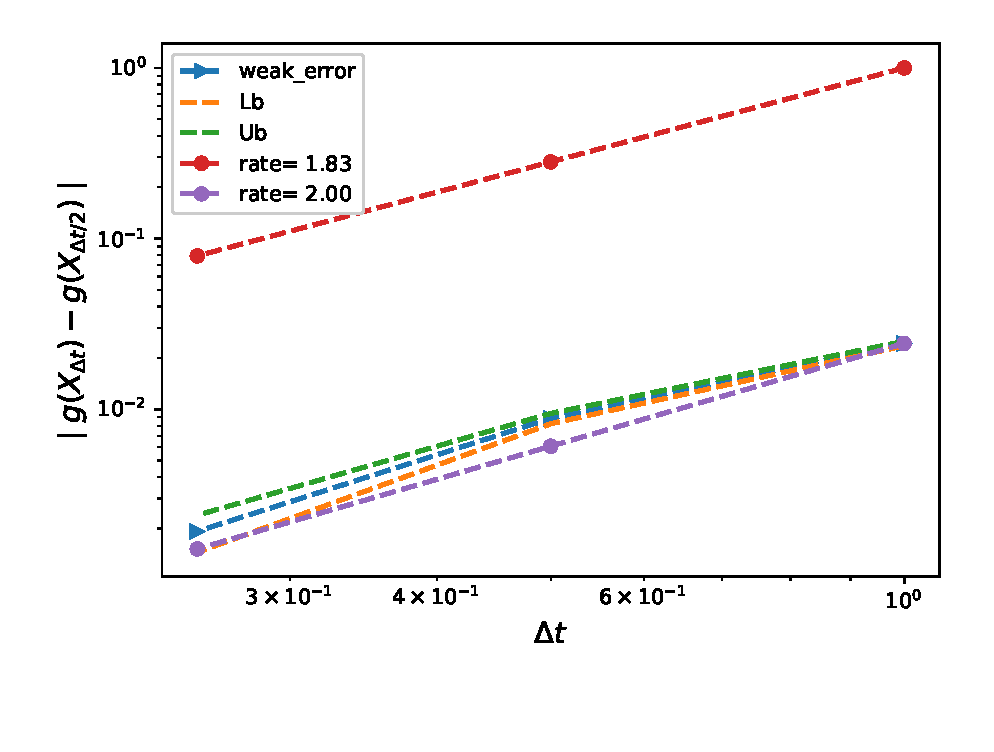
\includegraphics[width=1\linewidth]{./figures/weak_error_rates_call/Beta_10/with_richardson/weak_convergence_order_differences_call_richardson_relative_M_10_6}
%		\caption{}
%		\label{fig:sub4}
%	\end{subfigure}
%	
%	\caption{The rate of convergence of the weak error for the  call option with Richardson extraploation, using MC with $M=10^6$: a) $\abs{\expt{2 g(X_{\Delta t/2}) -g(X_{\Delta t})}-g(X)}$  b) $\abs{\expt{3 g(X_{\Delta t/2})-g(X_{\Delta t})-2 g(X_{\Delta t/4})}}$ }
%	\label{fig:fig:Weak_rate_call_with_rich}
%\end{figure}



%\begin{figure}[h!]
%	\centering
%	\begin{subfigure}{.4\textwidth}
%		\centering
%		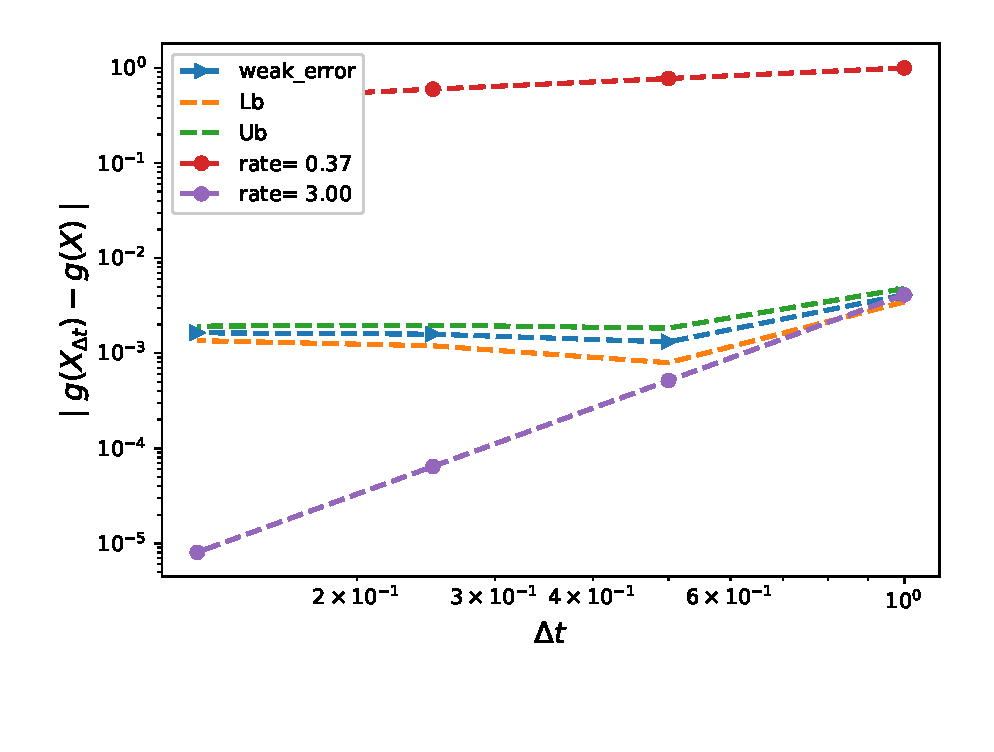
\includegraphics[width=1\linewidth]{./figures/weak_error_rates_call/Beta_10/with_richardson/weak_convergence_order_Call_richardson_level2_relative_M_10_6}
%		\caption{}
%		\label{fig:sub3}
%	\end{subfigure}%
%	\begin{subfigure}{.4\textwidth}
%		\centering
%		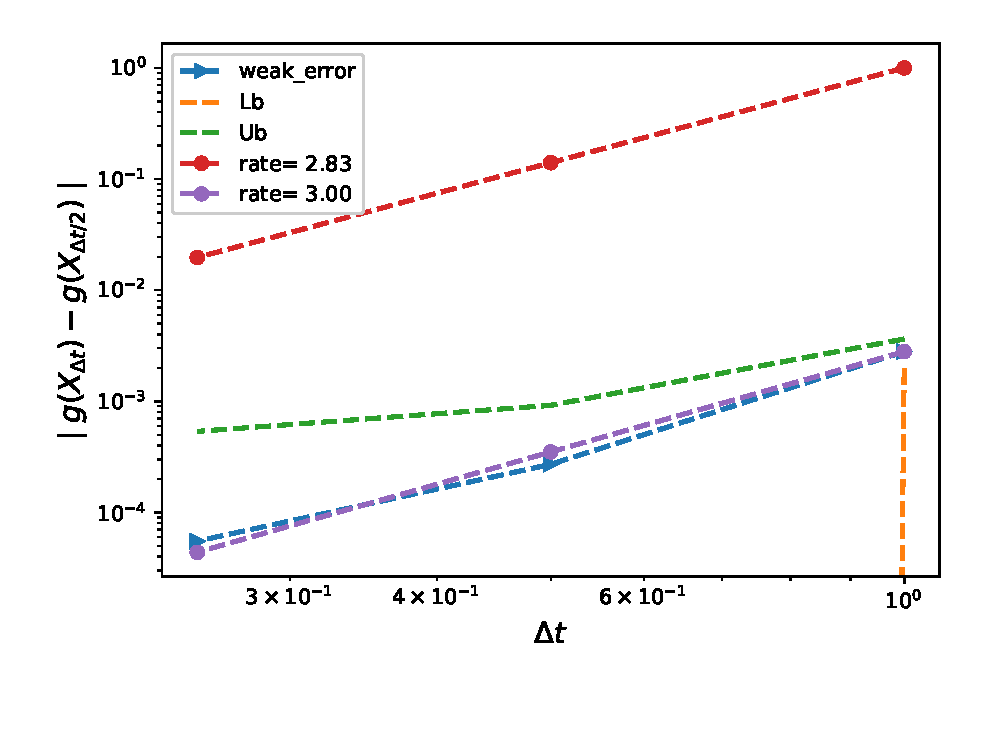
\includegraphics[width=1\linewidth]{./figures/weak_error_rates_call/Beta_10/with_richardson/weak_convergence_order_differences_Call_richardson_level2_relative_M_10_6}
%		\caption{}
%		\label{fig:sub4}
%	\end{subfigure}
	
%	\caption{The rate of convergence of the weak error for the  call option with Richardson extraploation (level 2), using MC with $M=10^6$: a) $\abs{\frac{1}{3}\expt{8 g(X_{\Delta t/4}) -6g(X_{\Delta t/2}) +g(X_{\Delta t})}-g(X)}$  b) $\abs{\frac{1}{3}\expt{-8 g(X_{\Delta t/8}) +14g(X_{\Delta t/4})-7 (X_{\Delta t/2}) +g(X_{\Delta t})}}$}
%	\label{fig:Weak_rate_call_with_rich_level2}
%\end{figure}


%\FloatBarrier
%\subsubsection*{$\beta=32$}

\begin{figure}[h!]
	\centering
%	\begin{subfigure}{.35\textwidth}
%		\centering
		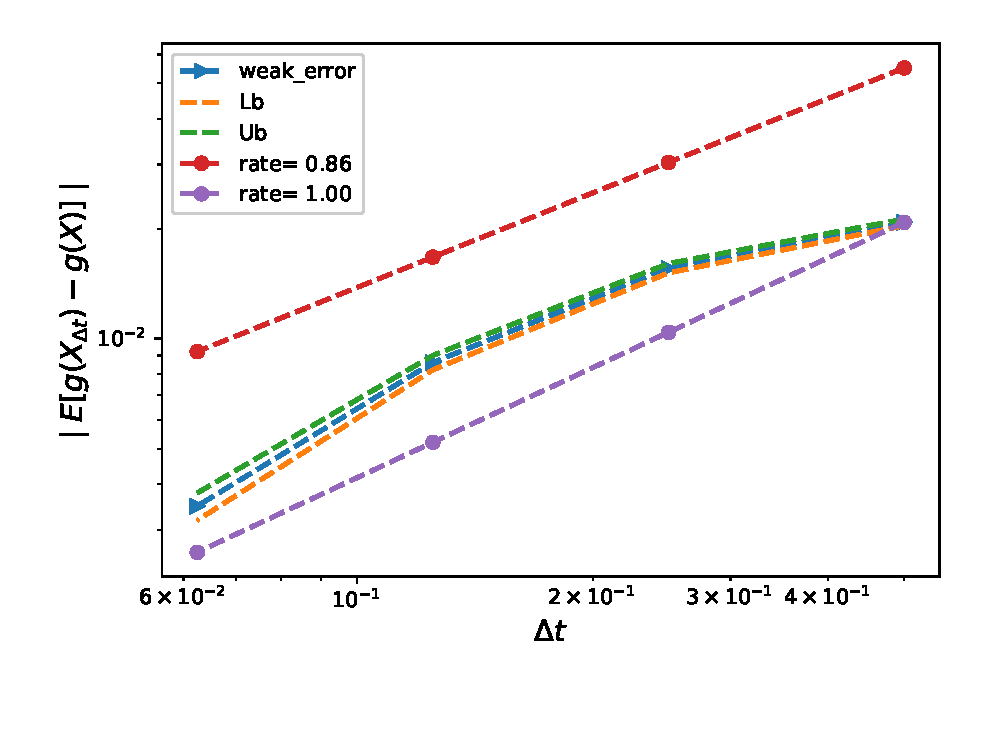
\includegraphics[width=0.5\linewidth]{./figures/weak_error_rates_call/Beta_32/without_rich/weak_convergence_order_call_option_relative_M_4_10_5}
%		\caption{}
%		\label{fig:sub3}
%	\end{subfigure}%
%	\begin{subfigure}{.35\textwidth}
%		\centering
%		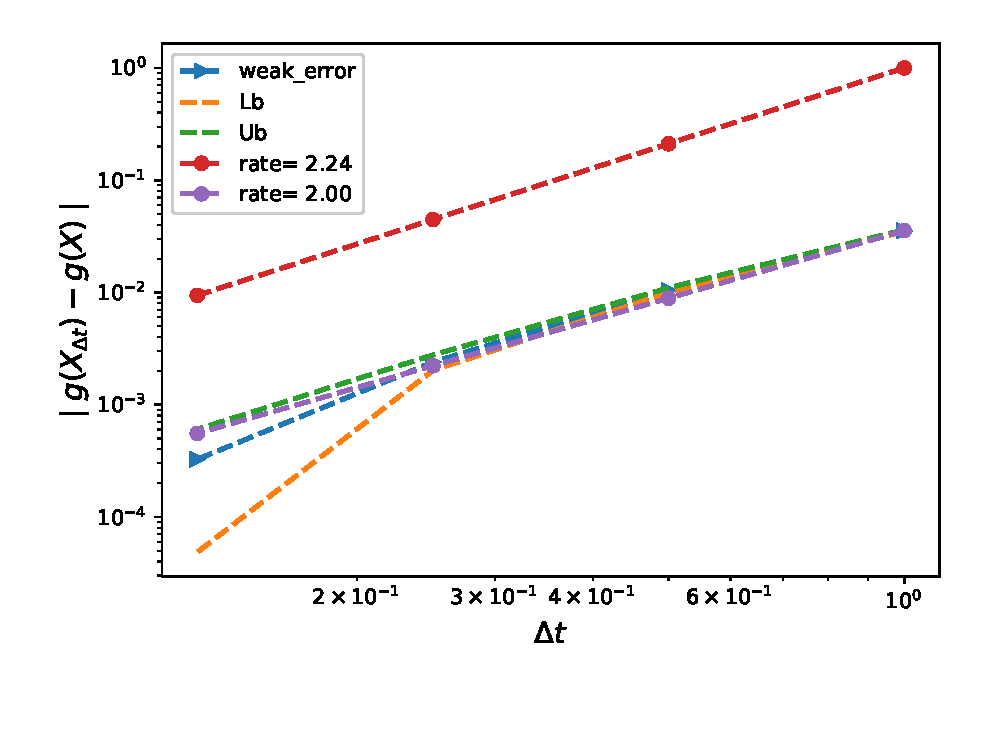
\includegraphics[width=1\linewidth]{./figures/weak_error_rates_call/Beta_32/with_rich/weak_convergence_order_call_richardson_relative}
%		\caption{}
%		\label{fig:sub4}
%	\end{subfigure}
	
	\caption{The convergence of the relative weak error  $\mathcal{E}_B(N)$ defined in \ref{eq:total_error}, using MC with $M=4 \times 10^5$ samples  for the call option example. The upper and lower bounds are $95\%$ confidence intervals.}
	\label{fig:Weak_rate_call_beta_32}
\end{figure}

%\begin{figure}[h!]
%	\centering
%	\begin{subfigure}{.35\textwidth}
%		\centering
%		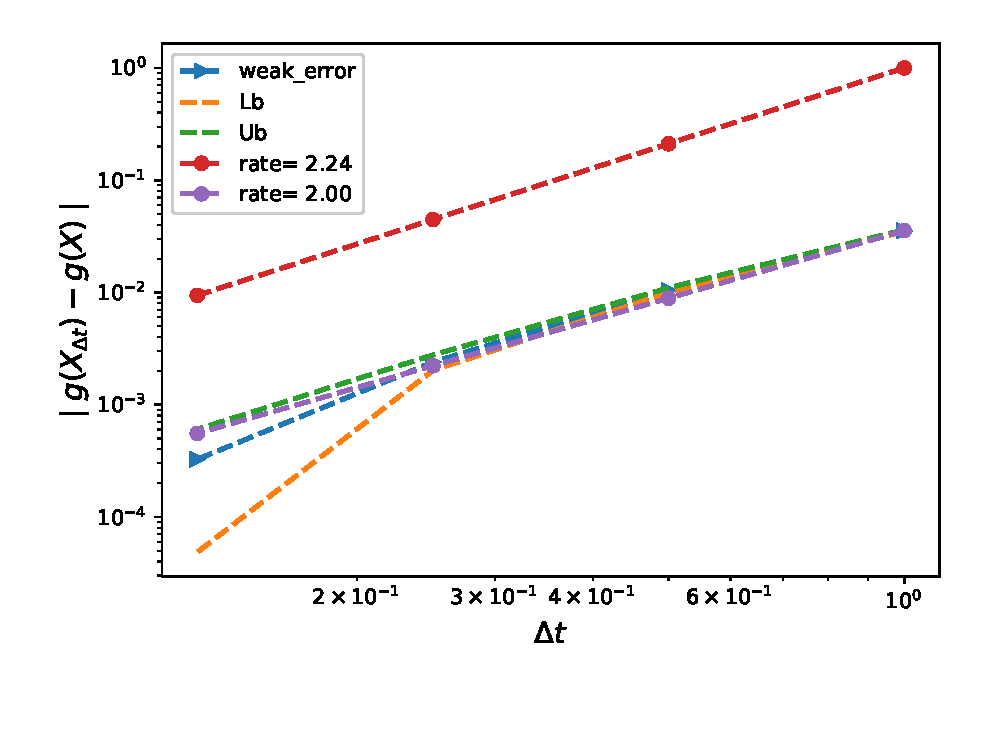
\includegraphics[width=1\linewidth]{./figures/weak_error_rates_call/Beta_32/with_rich/weak_convergence_order_call_richardson_relative}
%		\caption{}
%		\label{fig:sub3}
%	\end{subfigure}%
%	\begin{subfigure}{.35\textwidth}
%		\centering
%		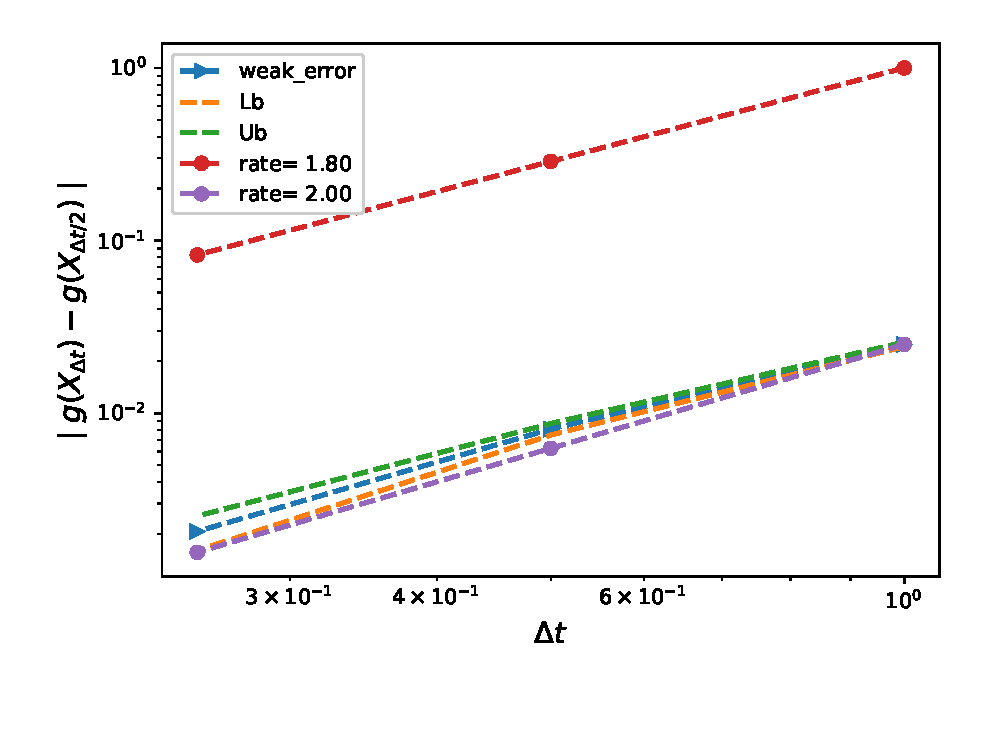
\includegraphics[width=1\linewidth]{./figures/weak_error_rates_call/Beta_32/with_rich/weak_convergence_order_differences_call_richardson_relative}
%		\caption{}
%		\label{fig:sub4}
%	\end{subfigure}
%	
%	\caption{The rate of convergence of the weak error for the  call option with Richardson extraploation (level 1), using MC with $M=5.10^6$: a)   b) $\abs{\expt{3 g(X_{\Delta t/2})-g(X_{\Delta t})-2 g(X_{\Delta t/4})}}$}
%	\label{fig:Weak_rate_call_with_rich_level1_beta_32}
%\end{figure}


%\begin{figure}[h!]
%	\centering
%	\begin{subfigure}{.4\textwidth}
%		\centering
%		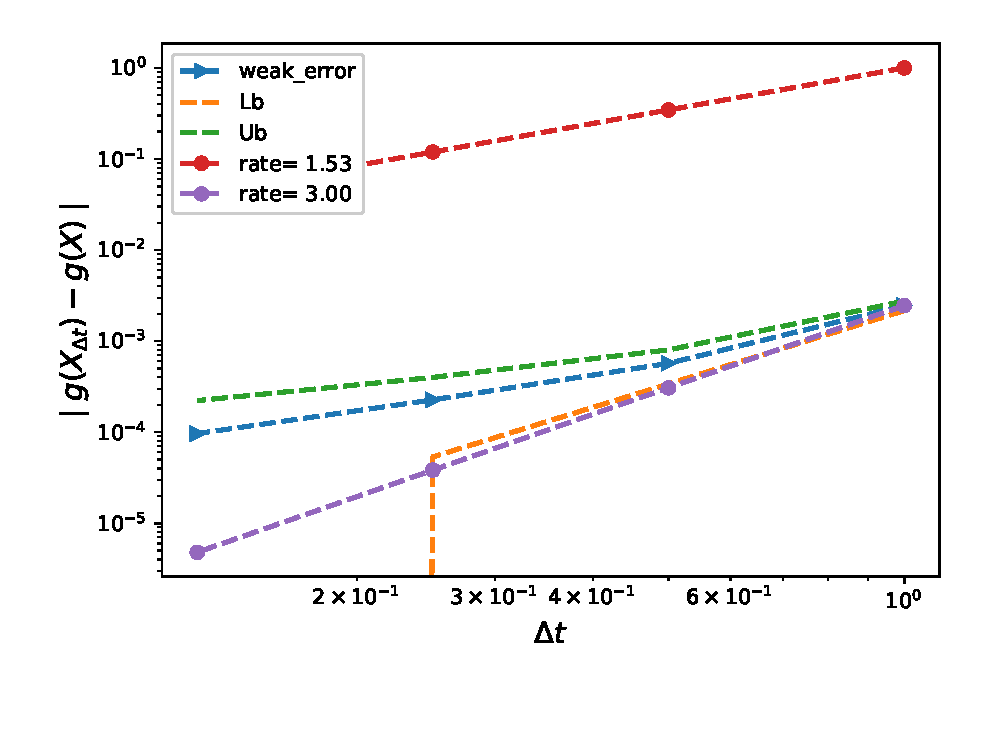
\includegraphics[width=1\linewidth]{./figures/weak_error_rates_call/Beta_32/with_rich/weak_convergence_order_Call_richardson_level2_relative_M_5_10_6}
%		\caption{}
%		\label{fig:sub3}
%	\end{subfigure}%
%	\begin{subfigure}{.4\textwidth}
%		\centering
%		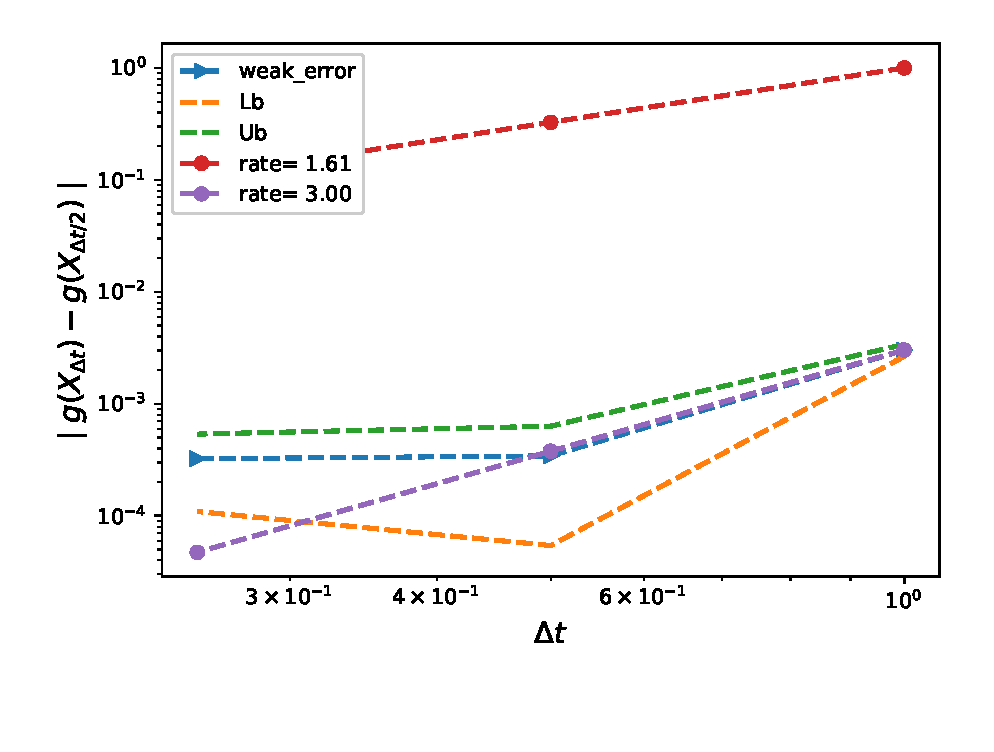
\includegraphics[width=1\linewidth]{./figures/weak_error_rates_call/Beta_32/with_rich/weak_convergence_order_differences_Call_richardson_level2_relative_M_5_10_6}
%		\caption{}
%		\label{fig:sub4}
%	\end{subfigure}
%	
%	\caption{The rate of convergence of the weak error for the  call option with Richardson extraploation (level 2), using MC with $M=5.10^6$: a) $\abs{\frac{1}{3}\expt{8 g(X_{\Delta t/4}) -6g(X_{\Delta t/2}) +g(X_{\Delta t})}-g(X)}$  b) $\abs{\frac{1}{3}\expt{-8 g(X_{\Delta t/8}) +14g(X_{\Delta t/4})-7 (X_{\Delta t/2}) +g(X_{\Delta t})}}$}
%	\label{fig:Weak_rate_call_with_rich_level2_beta_32}
%\end{figure}

\FloatBarrier
%\subsubsection{Comparing relative errors}\label{sec:Comparing relative errors, call}
%\subsubsection*{Without Richardson extrapolation}


%
%In this Section, we report the results for the Call option, using the different Methods: MISC, MC $+$ root finding  and MC, without Richardson extrapolation . We mention that for MISC we used a very small tolerance for the Newton solver, when solving the Kink point problem ($TOL_{\text{Newton}}=10^{-10}$), we also used $\beta=32$ (number of Laguerre quadrature points ). We start by reporting the observed approximated values using different methods (See table \ref{table:Call option price of the different methods for different number of time steps, without Richardson extrapolation.}). The biased values for MC method were computed using the values of Bias, reported in table \ref{Bias and Statistical errors of MC  for computing Call option price  for different number of time steps, without Richardson extrapolation. The numbers between parentheses are the corresponding absolute errors.}. In table \ref{Quadrature error of MISC to compute Call option price of the different tolerances for different number of time steps, without Richardson extrapolation. The numbers between parentheses are the corresponding absolute errors.}, we report the behavior of quadrature error with respect to MISC tolerance. We precise that the quadrature error is computed by substracting the MISC approximated value from the biased MC value. We report in red the values where MISC becomes stable (see also figure \ref{fig:Quadrature_error_non_rich_Call}). Those values where used to compute the needed number of samples for MC (with and without root finding), to achieve similar magnitude  for statistical error. Later, in table \ref{Total error of MISC and MC to compute Call option price of the different tolerances for different number of time steps, without Richardson extrapolation. The numbers between parentheses are the corresponding absolute errors.}, we report the total relative error for all methods (Quadrature error + Bias for MISC and Statistical error + Bias for MC). We also report in table \ref{Comparsion of the computational time of  MC and MISC, used to compute Call option price  for different number of time steps, without Richardson extrapolation}, the computational time needed for all different methods.  We finally provide in figure \ref{fig:Complexity plot for MC and MISC , Call non rich}, the complexity rates for the different involved methods.

%\begin{table}[h!]
%	\centering
%	\begin{tabular}{l*{6}{c}r}
%		Method \textbackslash  Steps            & $2$ & $4$ & $8$ & $16$ &   \\
%		\hline
%		MISC ($TOL_{\text{MISC}}=5.10^{-1},\beta=32$)  & $16.184$ & $16.070$ & $15.998$ & $15.930$  \\
%		MISC ($TOL_{\text{MISC}}=10^{-1},\beta=32$)  & $16.184$ & $16.070$ & $15.996$ &$15.928$  \\
%		MISC ($TOL_{\text{MISC}}=5.10^{-2},\beta=32$) & $16.184$ & $16.070$ & $15.996$ & $15.928$  \\
%		MISC ($TOL_{\text{MISC}}=10^{-2},\beta=32$) & $16.184$ & $16.103$ & $15.996$ &$15.928$  \\
%%		MISC ($TOL_{\text{MISC}}=10^{-3},\beta=32$) & $16.184$ & $16.103$ & $15.996$ & $-$  \\
%		
%		\hline
%		MC method ($M=10^{5}$)   & $  16.194$ & $ 16.099$ & $
%		15.999$ & $  15.923$  \\
%		\hline
%	\end{tabular}
%	\caption{Call option price of the different methods for different number of time steps, without Richardson extrapolation.}
%	\label{table:Call option price of the different methods for different number of time steps, without Richardson extrapolation.}
%\end{table}

%
%\begin{table}[h!]
%	\centering
%	\begin{tabular}{l*{6}{c}r}
%		Method \textbackslash  Steps            & $2$ & $4$ & $8$ & $16$  \\
%		\hline
%		MC Bias ($M=10^{5}$)  & 	$ \underset{(      0.3424 )}{\mathbf{0.0216}}$  & $\underset{(0.2473)}{\mathbf{ 0.0156
%		}}$  & $\underset{(  0.1474)}{\mathbf{0.0093}}$ & $\underset{(     0.0713
%	)}{\mathbf{  0.0045 }}$\\ 
%		
%		MC Statistical error  ($M=10^{5}$)   & 	$ \underset{( 7.5e-03  )}{\mathbf{4.4e-04}}$  & $\underset{(7.5e-03 )}{\mathbf{ 4.7e-04
%		}}$  & $\underset{(6.3e-03 )}{\mathbf{4.0e-04}}$ & $\underset{( 4.9e-03 )}{\mathbf{ 3.1e-04  }}$\\ 
%	
%%		MC Statistical error ($M=10^4$)     & 	$ \underset{( 2.2e-02  )}{\mathbf{1.4e-03}}$  & 	$ \underset{( 2.2e-02  )}{\mathbf{1.4e-03}}$  & $\underset{(1.9e-02 )}{\mathbf{1.2e-03}}$ & $\underset{( 1.5e-02 )}{\mathbf{ 9.3e-04  }}$\\ 
%%		
%		\hline
%	\end{tabular}
%	\caption{Bias and statistical errors of MC  for computing call option price  for different number of time steps, without Richardson extrapolation. The numbers between parentheses are the corresponding absolute errors.}
%	\label{Bias and Statistical errors of MC  for computing Call option price  for different number of time steps, without Richardson extrapolation. The numbers between parentheses are the corresponding absolute errors.}
%\end{table}



%
%\begin{table}[h!]
%	\centering
%	\begin{tabular}{l*{6}{c}r}
%		Method \textbackslash  Steps            & $2$ & $4$ & $8$ & $16$  \\
%		\hline
%		MISC ($TOL_{\text{MISC}}=5.10^{-1}$)  & $\underset{( 0.0103)}{\mathbf{\red{0.0007}}}$ & $\underset{(0.0290)}{\mathbf{0.0018}}$  & $\underset{(0.0010
%			)}{\mathbf{6.3e-05}}$ &$\underset{(   0.0070)}{\mathbf{0.0004}}$ \\
%		MISC ($TOL_{\text{MISC}}=10^{-1}$)   &  $\underset{( 0.0103)}{\mathbf{0.0007}}$& $\underset{(0.0290)}{\mathbf{0.0018}}$ & $\underset{(
%			0.0030
%			)}{\mathbf{\red{0.0002}}}$ &$\underset{(0.0020)}{\mathbf{\red{0.0001}}}$ \\
%		MISC ($TOL_{\text{MISC}}=5.10^{-2}$)  &$\underset{( 0.0103)}{\mathbf{0.0007}}$ & $\underset{(0.0290)}{\mathbf{0.0018}}$  & $\underset{(
%			0.0030
%			)}{\mathbf{0.0002}}$ &$\underset{(0.0020)}{\mathbf{0.0001}}$ \\
%		MISC ($TOL_{\text{MISC}}=10^{-2}$)  & $\underset{( 0.0103)}{\mathbf{0.0007}}$ & $\underset{( 0.0040)}{\mathbf{\red{0.0003}}}$  & $\underset{(
%			0.0030
%			)}{\mathbf{0.0002}}$ &$\underset{(0.0020)}{\mathbf{0.0001}}$ \\
%%		MISC ($TOL_{\text{MISC}}=10^{-3}$)  & $\underset{( 0.0103)}{\mathbf{0.0007}}$  & $\underset{( 0.0040)}{\mathbf{0.0003}}$ & $\underset{(
%%			0.0030
%%			)}{\mathbf{0.0002}}$ &$\underset{(-)}{\mathbf{-}}$ \\
%%		
%		\hline
%	\end{tabular}
%	\caption{Quadrature error of MISC, with different tolerances, to compute call option price for different number of time steps, without Richardson extrapolation. The numbers between parentheses are the corresponding absolute errors. The values marked in red correspond to stable quadrature errors for MISC, and will be used for complexity comparison against MC.}
%	\label{Quadrature error of MISC to compute Call option price of the different tolerances for different number of time steps, without Richardson extrapolation. The numbers between parentheses are the corresponding absolute errors.}
%\end{table}
%
%\FloatBarrier
%	\begin{figure}[h!]
%\centering
%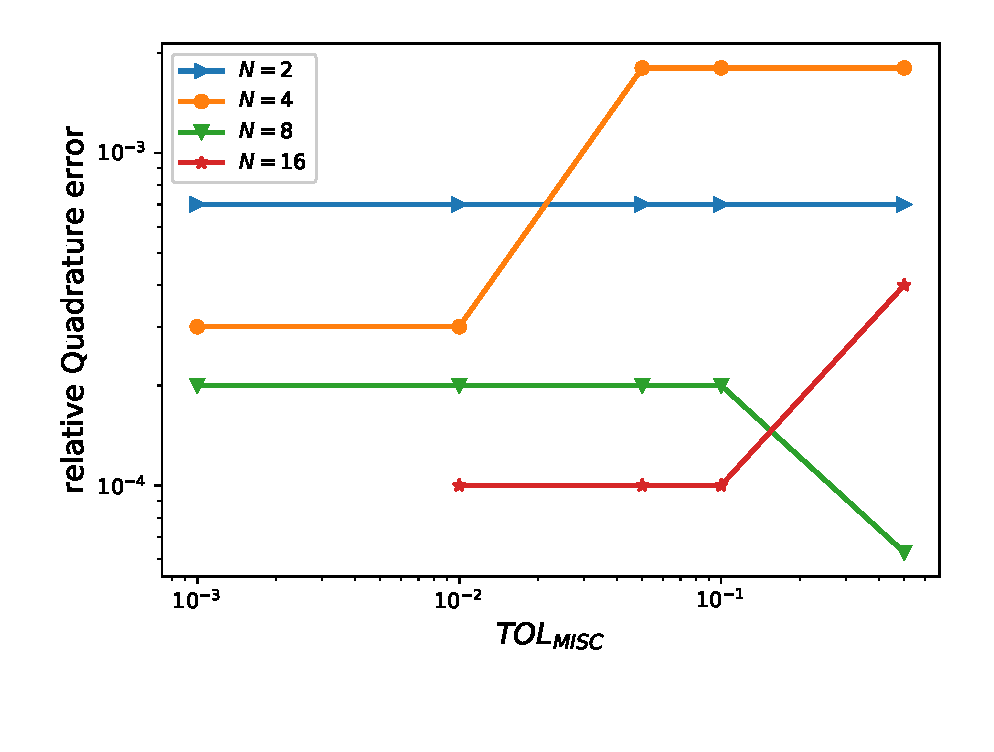
\includegraphics[width=0.4\linewidth]{./figures/Call_MISC_quadrature_error/relative_quad_error_wrt_MISC_TOL_non_rich}
%
%
%\caption{Relative quadrature error of MISC, with different tolerances, to compute call option price for different number of time steps, without Richardson extrapolation.}
%\label{fig:Quadrature_error_non_rich_Call}
%\end{figure}
%

\FloatBarrier
\begin{table}[h!]
	\centering
	\begin{tabular}{l*{6}{c}r}
		\toprule[1.5pt]
	Method & & Steps  & &     \\
	\hline
           & $2$ & $4$ & $8$ & $16$  \\
		\hline
%		($TOL_{\text{MISC}}=5.10^{-1}$, $\beta=32$)  
		MISC &  $\underset{(0.021,0.001)}{\mathbf{0.022}}$ & $\underset{(0.016,0.002)}{\mathbf{0.018}}$ & $\underset{(0.009,0.0001)}{\mathbf{0.009}}$ & $\underset{(0.004,0.0004)}{\mathbf{0.004}}$  \\
%		MISC ($TOL_{\text{MISC}}=10^{-1}$)  &  $\underset{(0.022,0.001)}{\mathbf{0.023}}$& $\underset{(0.016,0.002)}{\mathbf{0.018}}$ & $\underset{(0.009,0.0002)}{\mathbf{\red{0.009}}}$ & $\underset{(0.005,0.0001)}{\mathbf{\red{0.005}}}$  \\
%		MISC ($TOL_{\text{MISC}}=5.10^{-2}$) & $\underset{(0.022,0.001)}{\mathbf{0.0223}}$ & $\underset{(0.016,0.002)}{\mathbf{0.018}}$ &  $\underset{(0.009,0.0002)}{\mathbf{0.009}}$ & $\underset{(0.005,0.0001)}{\mathbf{0.005}}$  \\
%		MISC ($TOL_{\text{MISC}}=10^{-2}$)  &  $\underset{(0.022,0.001)}{\mathbf{0.023}}$& $\underset{(0.016,0.0003)}{\mathbf{\red{0.016}}}$ & $\underset{(0.009,0.0002)}{\mathbf{0.009}}$ &  $\underset{(0.005,0.0001)}{\mathbf{0.005}}$  \\
%		MISC ($TOL_{\text{MISC}}=10^{-3}$) &  $\mathbf{0.0223}$ & $\mathbf{0.0159}$ & $\mathbf{0.0095}$ & $\mathbf{}$  \\
		
		\hline
%		MC  ($M=10^5$)   &  $\mathbf{0.0266}$ & $\mathbf{0.0161}$ & $\mathbf{0.0097}$ & $\mathbf{\red{0.0048}}$  \\	
%		($\beta=32$) 
			MC +root finding  &  $\underset{(0.021,0.02)}{\mathbf{0.041}}$ & $\underset{(0.016,0.016)}{\mathbf{0.032}}$ & $\underset{(0.009,0.009)}{\mathbf{0.018}}$ & $\underset{(0.004,0.004)}{\mathbf{0.008}}$  \\
			M(\# MC samples)   & $10^2 $  & $3 \times 10^2 $  & $
			10^3$ & $4 \times 10^3$ \\	
		\hline	
				MC   &  $\underset{(0.02,0.02)}{\mathbf{0.04}}$ & $\underset{(0.016,0.016)}{\mathbf{0.032}}$ & $\underset{(0.01,0.01)}{\mathbf{}0.02}$ & $\underset{(0.004,0.004)}{\mathbf{0.008}}$  \\	
				M(\# MC samples)   & $3 \times 10^4$  & $5\times 10^4$  & $2\times 10^5$ & $8\times 10^5$ \\	
		
			\bottomrule[1.25pt]
	\end{tabular}
	\caption{Total relative  error of MISC, with different tolerances, and MC to compute call option price for different number of time steps, without Richardson extrapolation. The values between parentheses correspond to the different errors contributing to the total relative error: for MISC we report the bias and quadrature errors and for MC we report the bias and the statistical errors. The number of MC samples,$ M$, is chosen to satisfy \eqref{optimal_number_samples}.}
	\label{Total error of MISC and MC to compute Call option price of the different tolerances for different number of time steps, without Richardson extrapolation. The numbers between parentheses are the corresponding absolute errors.}
\end{table}

\FloatBarrier




\begin{table}[h!]
	\centering
	\begin{tabular}{l*{6}{c}r}
		\toprule[1.5pt]
	Method & & Steps  & &     \\
	\hline
	         & $2$ & $4$ & $8$ & $16$ &   \\
		\hline
%		($TOL_{\text{MISC}}=5.10^{-1}$, $\beta=32$)
		MISC  & $0.3$ & $3$ & $17$ & $473$  \\
%		MISC ($TOL_{\text{MISC}}=10^{-1}$)  & $0.3$ & $3$ & $\red{58}$ & $\red{656}$  \\
%		MISC ($TOL_{\text{MISC}}=5.10^{-2}$)   & $0.3$ & $3$ & $73$ & $731$  \\
%		MISC ($TOL_{\text{MISC}}=10^{-2}$)  & $0.3$ & $\red{6}$ & $108$ & $1972$  \\
%%		MISC ($TOL_{\text{MISC}}=10^{-3}$)   & $0.3$ & $28$ & $264$ & $-$  \\
%		\hline
%		MC method ($M=10^5, \beta=32$)    & $168$ & $216$ & $290$ & $\red{432}$  \\
%($\beta=32$) 
			MC +root finding  & $3$ & $16$ & $70$ & $408$  \\
				MC  & $3$ & $13$ & $76$ & $380$  \\
%		\hline
%		
%			Ratio of	$\text{(MC+root finding)}/\text{(MISC)}$ & $\red{ 4400}$ & $\red{   1400}$ & $\red{369}$ & $\red{ 107}$  \\
%		Ratio of	$(\text{MC})/(\text{MISC})$ & $\red{ 4800}$ & $\red{ 1665}$ & $\red{ 565}$ & $\red{ 241}$  \\
		\bottomrule[1.25pt]
	\end{tabular}
	\caption{Comparison of the computational time of  MC and MISC, used to compute call option price  for different number of time steps, without Richardson extrapolation. The average computational time of MC is computed over $10$ runs.}
	\label{Comparsion of the computational time of  MC and MISC, used to compute Call option price  for different number of time steps, without Richardson extrapolation}
\end{table}



\FloatBarrier
	\begin{figure}[h!]
\centering
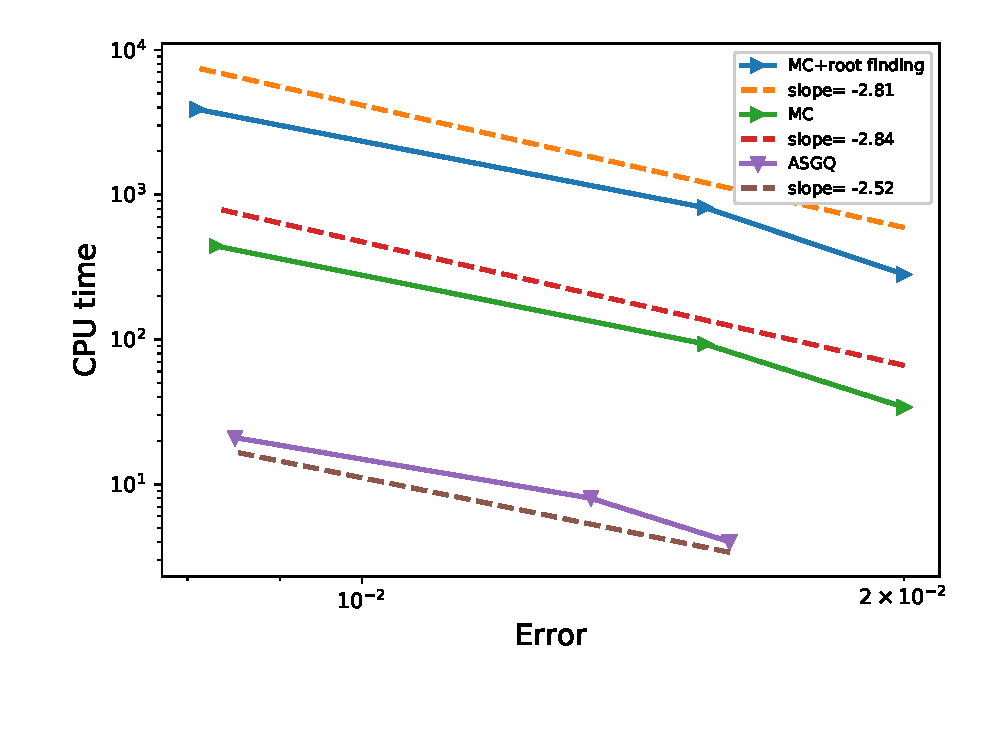
\includegraphics[width=0.4\linewidth]{./figures/Call_Complexity_rates/error_vs_time}

\caption{Computational work comparison for MISC and MC methods, for the case of  call option. This plot shows that to achieve a relative error below $1\%$, MISC outperforms significantly MC method in terms of computational time.}
\label{fig:Complexity plot for MC and MISC , Call non rich}
\end{figure}


\FloatBarrier

%\subsubsection*{With Richardson extrapolation (level $1$)}
%
%
%
%%%
%%%In this Section, we report the results for the Call option, using the different Methods: MISC, MC $+$ root finding  and MC, with Richardson extrapolation . We mention that for MISC we used a very small tolerance for the Newton solver, when solving the Kink point problem ($TOL_{\text{Newton}}=10^{-10}$), we also used $\beta=32$ (number of Laguerre quadrature points ). We start by reporting the observed approximated values using different methods (See table \ref{table: Call option price of the different methods for different number of time steps, with Richardson extrapolation (level1).}. The biased values for MC method were computed using the values of Bias, reported in table \ref{Bias and Statistical errors of MC  for computing Call option price  for different number of time steps, with Richardson extrapolation (level $1$). The numbers between parentheses are the corresponding absolute errors.}. In table \ref{Quadrature error of MISC to compute Call option price of the different tolerances for different number of time steps, with Richardson extrapolation (level $1$). The numbers between parentheses are the corresponding absolute errors.}, we report the behavior of quadrature error with respect to MISC tolerance. We precise that the quadrature error is computed by substracting the MISC approximated value from the biased MC value. We report in red the values where MISC becomes stable (see also figure \ref{fig:Quadrature_error_with_rich_Call}). Those values where used to compute the needed number of samples for MC (with and without root finding), to achieve similar magnitude  for statistical error. Later, in table \ref{Total error of MISC and MC to compute Call option price of the different tolerances for different number of time steps, with Richardson extrapolation (level $1$). The numbers between parentheses are the corresponding absolute errors.}, we report the total relative error for all methods (Quadrature error + Bias for MISC and Statistical error + Bias for MC). We also report in table\ref{Comparsion of the computational time of  MC and MISC, used to compute Call option price  for different number of time steps, with Richardson extrapolation (level $1$)}, the computational time needed for all different methods.  We finally provide in figure \ref{fig:Complexity plot for MC and MISC , Call, comparison}, the comparison between the two versions of MISC (without/with Richardson extrapolation).
%
%
%%
%%\begin{table}[h!]
%%	\centering
%%	\begin{tabular}{l*{6}{c}r}
%%		Method \textbackslash  Steps            & $1-2$ & $2-4$ & $4-8$ & $8-16$ &   \\
%%		\hline
%%		MISC ($TOL_{\text{MISC}}=5.10^{-1}$)  & $16.4108$ & $16.0254$ & $15.8912$ & $15.8621$  \\
%%		MISC ($TOL_{\text{MISC}}=10^{-1}$)  & $16.4108$ & $16.0254$ & $15.8883$ & $15.8603$  \\
%%		MISC ($TOL_{\text{MISC}}=5.10^{-2}$) & $16.4108$ & $16.0218$ & $15.8885$ & $15.8600$  \\
%%%		MISC ($TOL_{\text{MISC}}=10^{-2}$) & $16.4108$& $16.0218$ & $15.8888$ & $15.8595$  \\
%%%		MISC ($TOL_{\text{MISC}}=10^{-3}$) & $16.4108$ & $16.0207$ & $15.8885$ & $-$  \\
%%		
%%		\hline
%%		MC method ($M=5.10^{6}$)   & $  16.4147$ & $ 16.0184$ & $15.8900$ & $15.8567$  \\
%%		\hline
%%	\end{tabular}
%%	\caption{Call option price of the different methods for different number of time steps, with Richardson extrapolation (level $1$).}
%%	\label{table: Call option price of the different methods for different number of time steps, with Richardson extrapolation (level1).}
%%\end{table}
%
%%
%%\begin{table}[h!]
%%	\centering
%%	\begin{tabular}{l*{6}{c}r}
%%		Method \textbackslash  Steps            & $1-2$ & $2-4$ & $4-8$ & $8-16$  \\
%%		\hline
%%		MC Bias ($M=5.10^6$)   & 	$ \underset{(    0.5627
%%			 )}{\mathbf{0.0355}}$  & $\underset{(  0.1664)}{\mathbf{ 0.0105
%%		}}$  & $\underset{( 0.0380)}{\mathbf{0.0024}}$ & $\underset{( 0.0048
%%	 )}{\mathbf{ 0.0003  }}$\\ 
%%		
%%		MC Statistical error ($M=5.10^6$)     & 	$ \underset{(  4.4e-03 )}{\mathbf{2.8e-04}}$  & $\underset{(3.8e-03 )}{\mathbf{ 2.4e-04
%%		}}$  & $\underset{(3.0e-03)}{\mathbf{1.9e-04}}$ & $\underset{(2.2e-03 )}{\mathbf{ 1.4e-04  }}$\\ 
%%		
%%%			MC Statistical error ($M=10^5$)     & 	$ \underset{(  1.4e-02 )}{\mathbf{9.0e-04}}$  & $\underset{(1.3e-02)}{\mathbf{ 8.0e-04
%%%		}}$  & $\underset{(9.4e-03)}{\mathbf{5.9e-04}}$ & $\underset{( 7.1e-03 )}{\mathbf{ 4.5e-04  }}$\\ 
%%		\hline
%%	\end{tabular}
%%	\caption{Bias and statistical errors of MC  for computing Call option price  for different number of time steps, with Richardson extrapolation (level $1$). The numbers between parentheses are the corresponding absolute errors.}
%%	\label{Bias and Statistical errors of MC  for computing Call option price  for different number of time steps, with Richardson extrapolation (level $1$). The numbers between parentheses are the corresponding absolute errors.}
%%\end{table}
%
%
%
%%
%%\begin{table}[h!]
%%	\centering
%%	\begin{tabular}{l*{6}{c}r}
%%		Method \textbackslash  Steps            & $1-2$ & $2-4$ & $4-8$ & $8-16$  \\
%%		\hline
%%		MISC ($TOL_{\text{MISC}}=5.10^{-1}$)  & $\underset{(0.0039
%%			)}{\mathbf{ \red{2.5e-04}}}$ & $\underset{(0.0070)}{\mathbf{4.4e-04}}$  & $\underset{(0.0012
%%			)}{\mathbf{7.6e-05}}$ &$\underset{(0.0054)}{\mathbf{3.4e-04}}$ \\
%%		MISC ($TOL_{\text{MISC}}=10^{-1}$)   & $\underset{(0.0039
%%			)}{\mathbf{ 2.5e-04}}$ & $\underset{(0.0070)}{\mathbf{4.4e-04}}$  & $\underset{(  0.0017)}{\mathbf{1.1e-04}}$ &$\underset{(0.0036)}{\mathbf{\red{2.3e-04}}}$ \\
%%		MISC ($TOL_{\text{MISC}}=5.10^{-2}$)  & $\underset{(0.0039
%%			)}{\mathbf{ 2.5e-04}}$ & $\underset{(0.0034)}{\mathbf{\red{\red{2.1e-04}}}}$  & $\underset{(    0.0015)}{\mathbf{\red{9.5e-05}}}$ &$\underset{(0.0033)}{\mathbf{2.1e-04}}$ \\
%%%		MISC ($TOL_{\text{MISC}}=10^{-2}$)  & $\underset{(0.0039
%%%			)}{\mathbf{ 2.5e-04}}$ & $\underset{(0.0034)}{\mathbf{2.1e-04}}$  & $\underset{(0.0012
%%%			)}{\mathbf{7.6e-05}}$&$\underset{(0.0028
%%%			)}{\mathbf{1.7e-04}}$ \\
%%%		MISC ($TOL_{\text{MISC}}=10^{-3}$)  & $\underset{(0.0039
%%%			)}{\mathbf{ 2.5e-04}}$ & $\underset{(0.0023
%%%			)}{\mathbf{1.5e-04}}$   &$\underset{(    0.0015)}{\mathbf{9.5e-05}}$ & $\underset{()}{\mathbf{}}$ \\
%%		
%%		\hline
%%	\end{tabular}
%%	\caption{Quadrature error of MISC, with different tolerances, to compute call option price  for different number of time steps, with Richardson extrapolation (level $1$). The numbers between parentheses are the corresponding absolute errors. The values marked in red correspond to stable quadrature errors for MISC, and will be used for complexity comparison against MC.}
%%	\label{Quadrature error of MISC to compute Call option price of the different tolerances for different number of time steps, with Richardson extrapolation (level $1$). The numbers between parentheses are the corresponding absolute errors.}
%%\end{table}
%
%%\FloatBarrier
%%
%%
%%	\begin{figure}[h!]
%%\centering
%%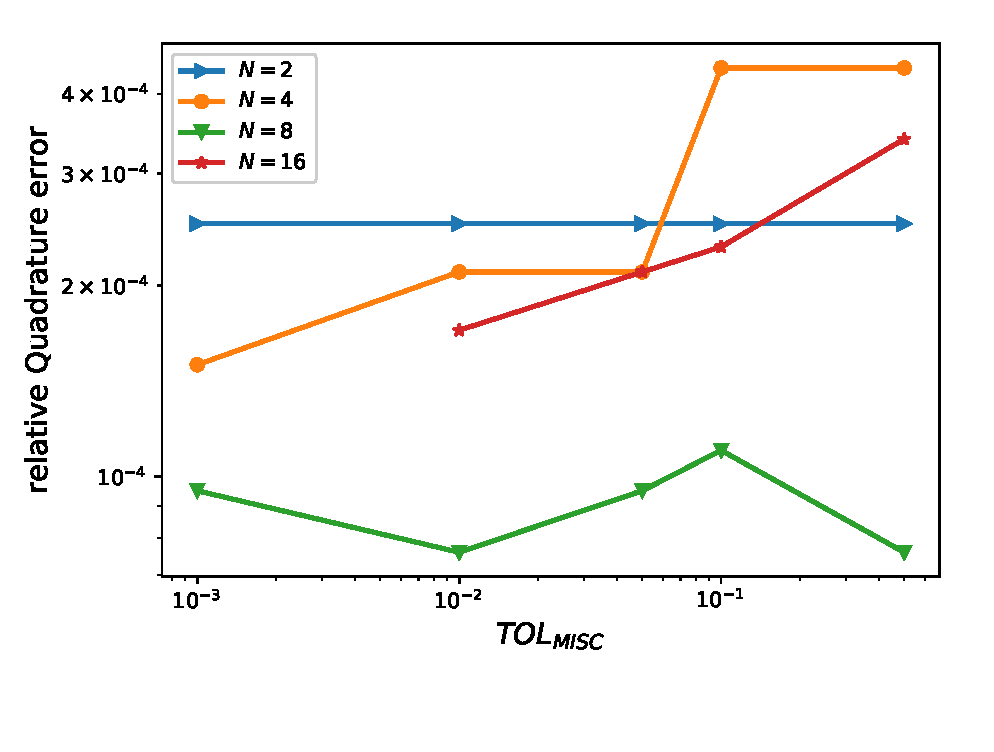
\includegraphics[width=0.4\linewidth]{./figures/Call_MISC_quadrature_error/relative_quad_error_wrt_MISC_TOL_with_rich}
%%
%%
%%\caption{Relative quadrature error of MISC, with different tolerances, to compute call option price for different number of time steps, with Richardson extrapolation.}
%%\label{fig:Quadrature_error_with_rich_Call}
%%\end{figure}
%%
%
%
%
%\FloatBarrier
%
%\begin{table}[h!]
%	\centering
%	\begin{tabular}{l*{6}{c}r}
%		\toprule[1.5pt]
%	Method & & Steps  &  &   \\
%	\hline
%	           & $1-2$ & $2-4$ & $4-8$ & $8-16$  \\
%		\hline
%		MISC ($TOL_{\text{MISC}}=5.10^{-1}$)  &  $\underset{(0.036,0.0003)}{\mathbf{0.036}}$ & $\underset{(0.011,0.0004)}{\mathbf{0.011}}$ & $\underset{(0.002,0.0001)}{\mathbf{0.002}}$ & $\underset{(0.0003,0.0003)}{\mathbf{0.0006}}$  \\
%%		MISC ($TOL_{\text{MISC}}=10^{-1}$)  &  $\underset{(0.036,0.0003)}{\mathbf{0.036}}$ & $\underset{(0.011,0.0004)}{\mathbf{0.011}}$ & $\underset{(0.002,0.0001)}{\mathbf{0.002}}$ & $\underset{(0.0003,0.0002)}{\mathbf{\red{0.0005}}}$  \\
%%		MISC ($TOL_{\text{MISC}}=5.10^{-2}$) &  $\underset{(0.036,0.0003)}{\mathbf{0.036}}$ & $\underset{(0.011,0.0002)}{\mathbf{\red{0.011}}}$ & $\underset{(0.002,0.0001)}{\mathbf{\red{0.002}}}$ & $\underset{(0.0003,0.0002)}{\mathbf{0.0005}}$  \\
%%		MISC ($TOL_{\text{MISC}}=10^{-2}$)  &  $\mathbf{0.0358}$ & $\mathbf{0.0107}$ & $\mathbf{0.0025}$ & $\mathbf{0.0005}$ \\
%%		MISC ($TOL_{\text{MISC}}=10^{-3}$) &  $\mathbf{0.0358}$ & $\mathbf{0.0107}$ & $\mathbf{0.0025}$ & $\mathbf{}$  \\
%		
%%		\hline
%%		MC  ($M=5.10^6$)   &  $\mathbf{\red{0.0358}}$ & $\mathbf{\red{0.0107}}$ & $\mathbf{\red{0.0026}}$ & $\mathbf{\red{0.0004}}$  \\	
%%			MC + root finding  &  $\mathbf{\red{0.0358}}$ & $\mathbf{\red{0.0107}}$ & $\mathbf{\red{0.0025}}$ & $\mathbf{\red{0.}}$  \\	
%		\bottomrule[1.25pt]
%	\end{tabular}
%	\caption{Total relative error of MISC, with different tolerances,  to compute call option price for different number of time steps, with Richardson extrapolation (level $1$).  The values marked in red, for MISC method, correspond to the total relative errors associated with  stable quadrature errors for MISC, and will be used for complexity comparison against MC.}
%	\label{Total error of MISC and MC to compute Call option price of the different tolerances for different number of time steps, with Richardson extrapolation (level $1$). The numbers between parentheses are the corresponding absolute errors.}
%\end{table}
%
%
%
%\FloatBarrier
%
%
%\begin{table}[h!]
%	\centering
%	\begin{tabular}{l*{6}{c}r}
%		\toprule[1.5pt]
%	Method & & Steps  &  &   \\
%	\hline
%         & $1-2$ & $2-4$ & $4-8$ & $8-16$ &   \\
%		\hline
%		MISC ($TOL_{\text{MISC}}=5.10^{-1}$) & $0.3$ & $4$ & $56$ & $713$  \\
%%		MISC ($TOL_{\text{MISC}}=10^{-1}$)  & $0.3$  & $4$ & $107$ & $\red{1126}$  \\
%%		MISC ($TOL_{\text{MISC}}=5.10^{-2}$)   & $0.3$  & $\red{9}$ & $\red{135}$ & $1253$  \\
%%%		MISC ($TOL_{\text{MISC}}=10^{-2}$)  &  $0.3$  & $9$ & $186$ & $3540$  \\
%%%		MISC ($TOL_{\text{MISC}}=10^{-3}$)   & $0.3$  & $63$ & $836$ & $$  \\
%%		\hline
%%		MC +root finding   & $\red{ 2.4e+05}$ & $\red{ 4.3e+05}$ & $\red{ 3.5e+06}$ & $\red{-}$  \\
%	\bottomrule[1.25pt]
%	\end{tabular}
%	\caption{Comparison of the computational time of  MISC, used to compute call option price  for different number of time steps, with Richardson extrapolation (level $1$). The average computational time of MC is computed over $10$ runs.}
%	\label{Comparsion of the computational time of  MC and MISC, used to compute Call option price  for different number of time steps, with Richardson extrapolation (level $1$)}
%\end{table}
%
%%	\begin{figure}[h!]
%%	\centering
%%	\includegraphics[width=0.7\linewidth]{./figures/Call_Complexity_rates/error_vs_time_rich}
%%	
%%	\caption{Complexity plot for MC and MISC for the case with Richardson extrapolation.}
%%	\label{fig:Complexity plot for MC and MISC , Call, with rich}
%%\end{figure}
%
%
%\FloatBarrier
%\begin{figure}[h!]
%	\centering
%	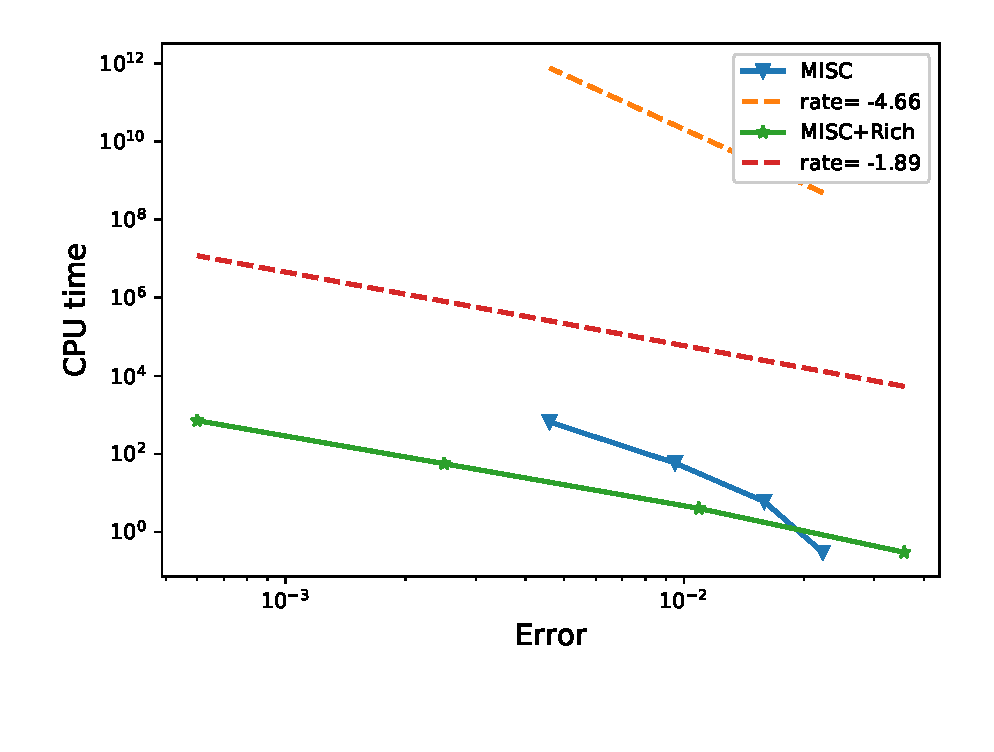
\includegraphics[width=0.4\linewidth]{./figures/Call_Complexity_rates/error_vs_time_comparision}
%	
%	\caption{Complexity plot for MISC without and with Richardson extrapolation, for the call option.}
%	\label{fig:Complexity plot for MC and MISC , Call, comparison}
%\end{figure}
%\FloatBarrier
%
%
%
%
%%In the following, we compare the  relative errors for the call option example under Black-Scholes model(see Tables (\ref{Relative error of the call option price of the different tolerances for different number of time steps.}, \ref{Relative error of Call option price of the different tolerances for different number of time steps, using Richardson extrapolation (level $1$)}, \ref{Relative error of Call option price of the different tolerances for different number of time steps, using Richardson extrapolation (level $2$)})). We report the results for $3$ scenarios: i) Without using Richardson extrapolation, ii) Using level $1$ Richardson extrapoaltion, iii) Using level $2$ Richardson extrapoaltion.  You may see appendix \ref{appendix:Call prices for different methods} for the values of call option prices. The value of $\beta$ used to get those points is $\beta=10$.
%%
%%Given the normalized bias computed by MC method (See Section \ref{sec:Weak error plots_call}) (reported as bold values in the tables), we report in red in each table the smallest tolerance that MISC required to get below that relative bias (I do not put values for smaller tolerances, once the required bias is reached). In case I do not reach those bias I put the best value that I get with MISC in red.
%%
%%From the tables (\ref{Relative error of the call option price of the different tolerances for different number of time steps.}, \ref{Relative error of Call option price of the different tolerances for different number of time steps, using Richardson extrapolation (level $1$)}, \ref{Relative error of Call option price of the different tolerances for different number of time steps, using Richardson extrapolation (level $2$)})), we may observe that to get a relative error below $0.5\%$, we need more than $16$ time steps for the case without Richardson extrapolation compared to only using $4$ time step in the coarse level for the case of level $1$ Richardson extraplation,  and  only using $1$ time step in the coarse level for the case of level $2$ Richardson extraplation.
%
%%\begin{table}[h!]
%%	\centering
%%	\begin{tabular}{l*{6}{c}r}
%%		Method \textbackslash  Steps            & $2$ & $4$ & $8$ & $16$ &   \\
%%		\hline
%%		MISC ($TOL_{\text{MISC}}=5.10^{-1}$)  & $ \red{0.0229}$ & $  0.0179$ & $\red{0.0111}$ & $ 0.0068$  \\
%%		MISC ($TOL_{\text{MISC}}=10^{-3}$)  & $-$ & $ \red{ 0.0177}$ & $-$ & $\red{  0.0066}$  \\
%%			MC method ($M=10^{5}$)&$ \mathbf{0.0231}$    & $\mathbf{0.0175}$  & $\mathbf{0.0111}$  & $\mathbf{0.0064}$ \\	
%%		\hline
%%	\end{tabular}
%%	\caption{Relative error of the call option price of the different tolerances for different number of time steps, without Richardson extrapolation}
%%	\label{Relative error of the call option price of the different tolerances for different number of time steps.}
%%\end{table}
%
%%\begin{table}[h!]
%%	\centering
%%	\begin{tabular}{l*{5}{c}r}
%%		Method \textbackslash  Steps    &$1-2$        & $2-4$ & $4-8$ & $8-16$  \\
%%		\hline
%%		MISC ($TOL_{\text{MISC}}=5.10^{-1}$)  &$\red{0.0372}$ & $ 0.0129$ & $0.0043$ & $ 0.0025$  \\
%%		MISC ($TOL_{\text{MISC}}=10^{-3}$) & $-$ & $ \red{0.0126}$ & $\red{    0.0042}$ & $\red{0.0023}$   \\
%%		MC method ($M=10^{5}$)&$ \mathbf{0.0374}$    & $\mathbf{0.0116}$  & $\mathbf{0.0027}$  & $\mathbf{0.0022}$ \\
%%		\hline
%%	\end{tabular}
%%	\caption{Relative error of the call option price of the different tolerances for different number of time steps, using Richardson extrapolation (level $1$)}
%%	\label{Relative error of Call option price of the different tolerances for different number of time steps, using Richardson extrapolation (level $1$)}
%%\end{table}
%
%
%%\begin{table}[h!]
%%	\centering
%%	\begin{tabular}{l*{5}{c}r}
%%		Method \textbackslash  Steps    &$1-2-4$        & $2-4-8$ & $4-8-16$   \\
%%		\hline
%%		MISC ($TOL_{\text{MISC}}=5.10^{-1}$)  &$0.0047$ & $  0.0015$ & $0.0019
%%		$   \\
%%		MISC ($TOL_{\text{MISC}}=10^{-3}$) & $ \red{0.0043}$ & $ \red{0.0013}$ & $\red{  0.0017}$    \\
%%		MC method ($M=10^{6}$)&$ \mathbf{0.0041}$    & $\mathbf{0.0013}$  & $\mathbf{0.0016}$  \\
%%		\hline
%%	\end{tabular}
%%	\caption{Relative error of the call option price of the different tolerances for different number of time steps, using Richardson extrapolation (level $2$)}
%%	\label{Relative error of Call option price of the different tolerances for different number of time steps, using Richardson extrapolation (level $2$)}
%%\end{table}
%
%


\subsection{The basket call option  under GBM  model}\label{sec:The basket call option  under GBM  model}
The third example that we consider  is the multi-dimensional  basket call option under GBM. 
\subsection{$d=2$}
For illustration, we start with the two dimensional basket call option  with parameters:  $S_0^{1,2}=K=100$, $\sigma_{1,2}=0.4$, $\rho=0.3$, $T=1$ $r=0$ and $c_{1,2}=1/2$, the reference value for those parameters  is  $12.90$. Figure \ref{fig:Weak_rate_two_dim_basket} shows the estimated   weak error  for the case without Richardson extrapolation, and we report the results for comparing MC and MISC in Tables \ref{Total error of MISC and MC to compute two  dim basket  Call option price of the different tolerances for different number of time steps, without Richardson extrapolation. The numbers between parentheses are the corresponding absolute errors.} and \ref{Comparsion of the computational time of  MC and MISC, used to compute two dim basket Call option price  for different number of time steps, without Richardson extrapolation}, and Figure \ref{fig:Complexity plot for MC and MISC , two dim basket call non rich}. Our numerical experiments show that MISC  requires approximately $5\%$ of the work of MC  to achieve a total relative error of around $0.9\%$.

\FloatBarrier
\begin{figure}[h!]
		\centering
		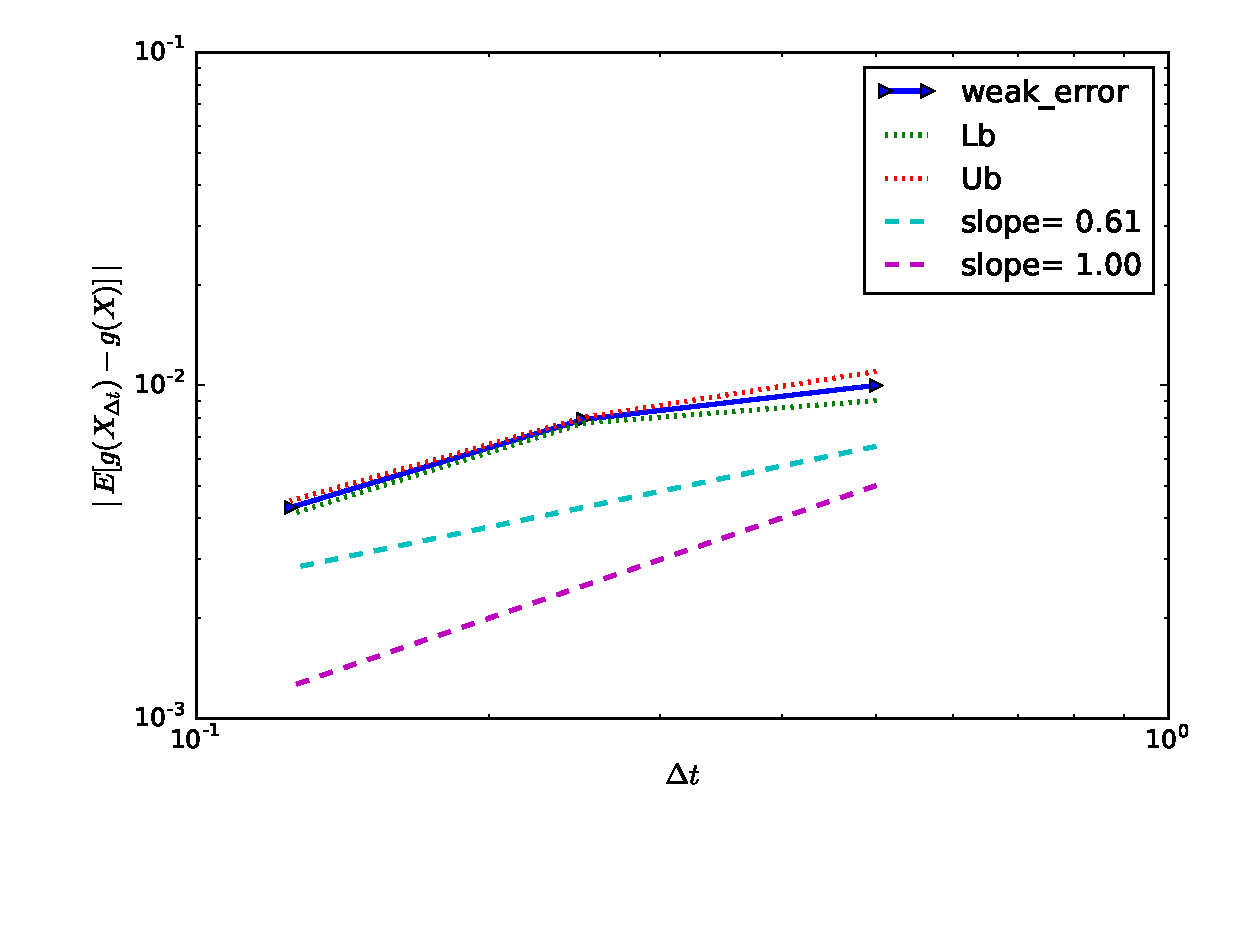
\includegraphics[width=0.4\linewidth]{./figures/basket_call_2d_time_stepping/weak_convergence/weak_convergence_order_basket_option_2d_relative_M_10_7_beta_128}

	\caption{The convergence of the relative weak error  $\mathcal{E}_B(N)$ defined in \ref{eq:total_error}, for the two dimensional basket call option with  a number of Laguerre  quadrature points  $\beta=128$ and number of samples for MC $M=10^7$. The upper and lower bounds are $95\%$ confidence intervals.}
	\label{fig:Weak_rate_two_dim_basket}
\end{figure}
\FloatBarrier


\FloatBarrier
\begin{table}[h!]
	\centering
	\begin{tabular}{l*{6}{c}r}
		\toprule[1.5pt]
	Method & & Steps  & &     \\
	\hline
           & $2$ & $4$ & $8$   \\
		\hline
		MISC   &  $\underset{(0.01,0.006)}{\mathbf{0.016}}$ & $\underset{(0.0079,0.0055)}{\mathbf{0.0134}}$ & $\underset{(0.0043,0.0042)}{\mathbf{0.0085}}$   \\

		\hline		
			MC +root finding   &  $\underset{(0.01,0.01)}{\mathbf{0.02}}$ & $\underset{(0.0079,0.0076)}{\mathbf{0.0155}}$ & $\underset{(0.0043,0.0038)}{\mathbf{0.0081}}$  \\
			M(\# MC samples)   & $2 \times 10^3$   &  $5 \times 10^3$ & $2 \times 10^4$  \\	
		\hline	
				MC   &  $\underset{(0.01,0.01)}{\mathbf{0.02}}$ & $\underset{(0.0079,0.0076)}{\mathbf{0.0155}}$ & $\underset{(0.0043,0.004)}{\mathbf{0.0083}}$   \\	
				M(\# MC samples)   &$10^5$  & $2 \times 10^5$  &  $8 \times 10^5$\\	
		
			\bottomrule[1.25pt]
	\end{tabular}
	\caption{Total relative  error of MISC, with different tolerances, and MC to compute two dimensional basket call option price for different number of time steps, without Richardson extrapolation. The values between parentheses correspond to the different errors contributing to the total relative error: for MISC we report the bias and quadrature errors and for MC we report the bias and the statistical errors. The number of MC samples,$ M$, is chosen to satisfy \eqref{optimal_number_samples}.}
	\label{Total error of MISC and MC to compute two  dim basket  Call option price of the different tolerances for different number of time steps, without Richardson extrapolation. The numbers between parentheses are the corresponding absolute errors.}
\end{table}
\FloatBarrier




\begin{table}[h!]
	\centering
	\begin{tabular}{l*{6}{c}r}
		\toprule[1.5pt]
	Method & & Steps  & &     \\
	\hline
	         & $2$ & $4$ & $8$    \\
		\hline
		MISC & $4$  & $8$ & $21$     \\
			MC +root finding  & $281$&  $814$&  $3888$   \\
				MC  &   $34$& $93$ &   $ 442$ \\
		\bottomrule[1.25pt]
	\end{tabular}
	\caption{Comparison of the computational time of  MC and MISC, used to compute two dimensional basket call option price  for different number of time steps, without Richardson extrapolation. The average computational time of MC is computed over $10$ runs.}
	\label{Comparsion of the computational time of  MC and MISC, used to compute two dim basket Call option price  for different number of time steps, without Richardson extrapolation}
\end{table}


\FloatBarrier
	\begin{figure}[h!]
\centering
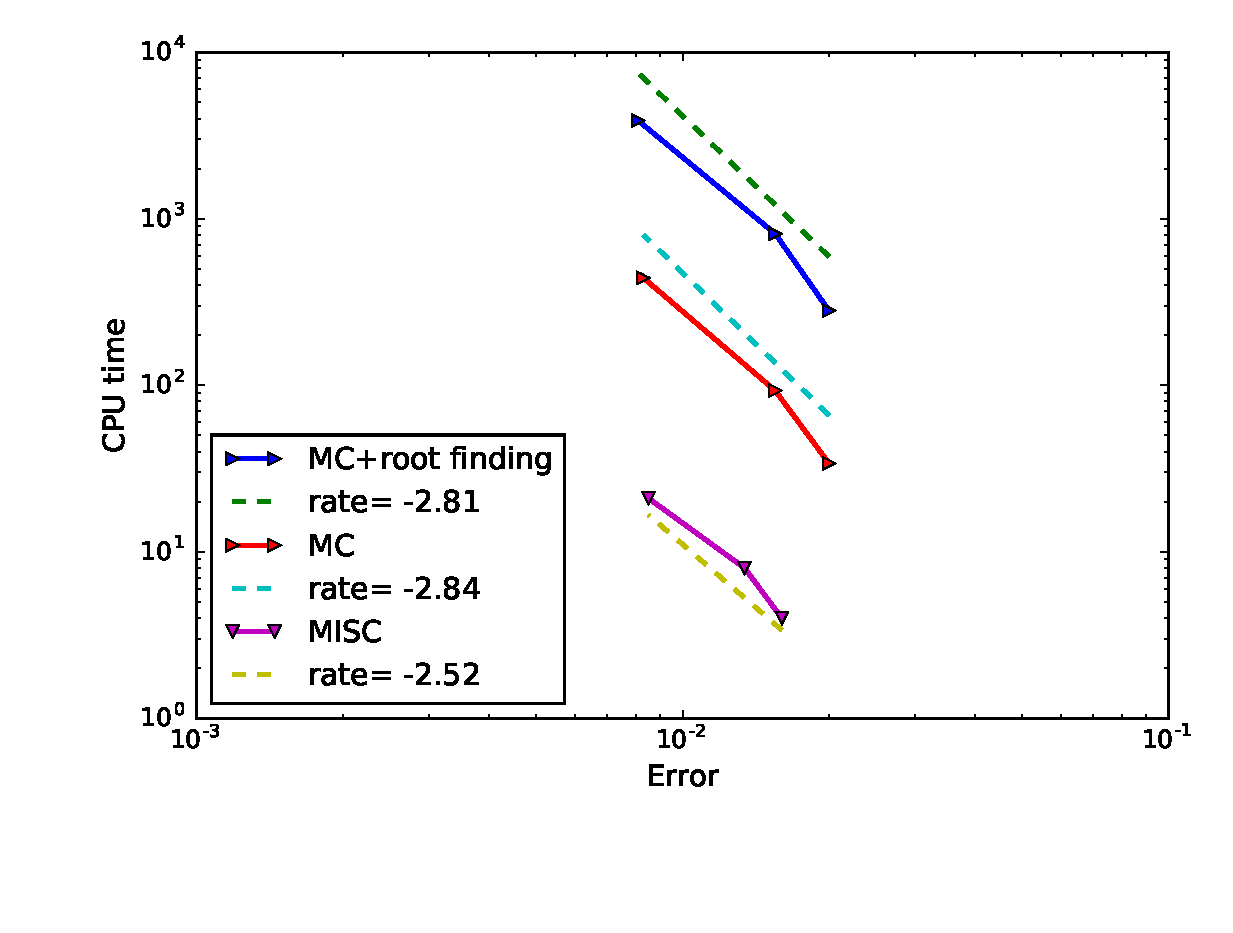
\includegraphics[width=0.4\linewidth]{./figures/basket_call_2d_time_stepping/complexity_rates/error_vs_time}

\caption{Computational work comparison for MISC and MC methods, for the case of two dimensional basket call option. This plot shows that to achieve a relative error below $1\%$, MISC outperforms significantly MC method in terms of computational time.}
\label{fig:Complexity plot for MC and MISC , two dim basket call non rich}
\end{figure}


\FloatBarrier

\subsection{$d=4$}
We consider now  the four dimensional basket call option  with parameters:  $S_0^{1,2,3,4}=K=100$, $\sigma_{1,2,3,4}=0.4$, $\rho=0.3$, $T=1$ $r=0$ and $c_{1,2,3,4}=1/4$, the reference value for those parameters  is  $11.04$. Figure \ref{fig:Weak_rate_4_dim_basket} shows the estimated   weak error  for the case without Richardson extrapolation, and we report the results for comparing MC and MISC in Tables \ref{Total error of MISC and MC to compute 4 dim basket  Call option price of the different tolerances for different number of time steps, without Richardson extrapolation. The numbers between parentheses are the corresponding absolute errors.} and \ref{Comparsion of the computational time of  MC and MISC, used to compute 4 dim basket Call option price  for different number of time steps, without Richardson extrapolation}, and Figure \ref{fig:Complexity plot for MC and MISC , 4 dim basket call non rich}.  Our numerical experiments show that MISC  requires approximately $4\%$ of the work of MC  to achieve a total relative error of around $0.8\%$.

\FloatBarrier
\begin{figure}[h!]
		\centering
		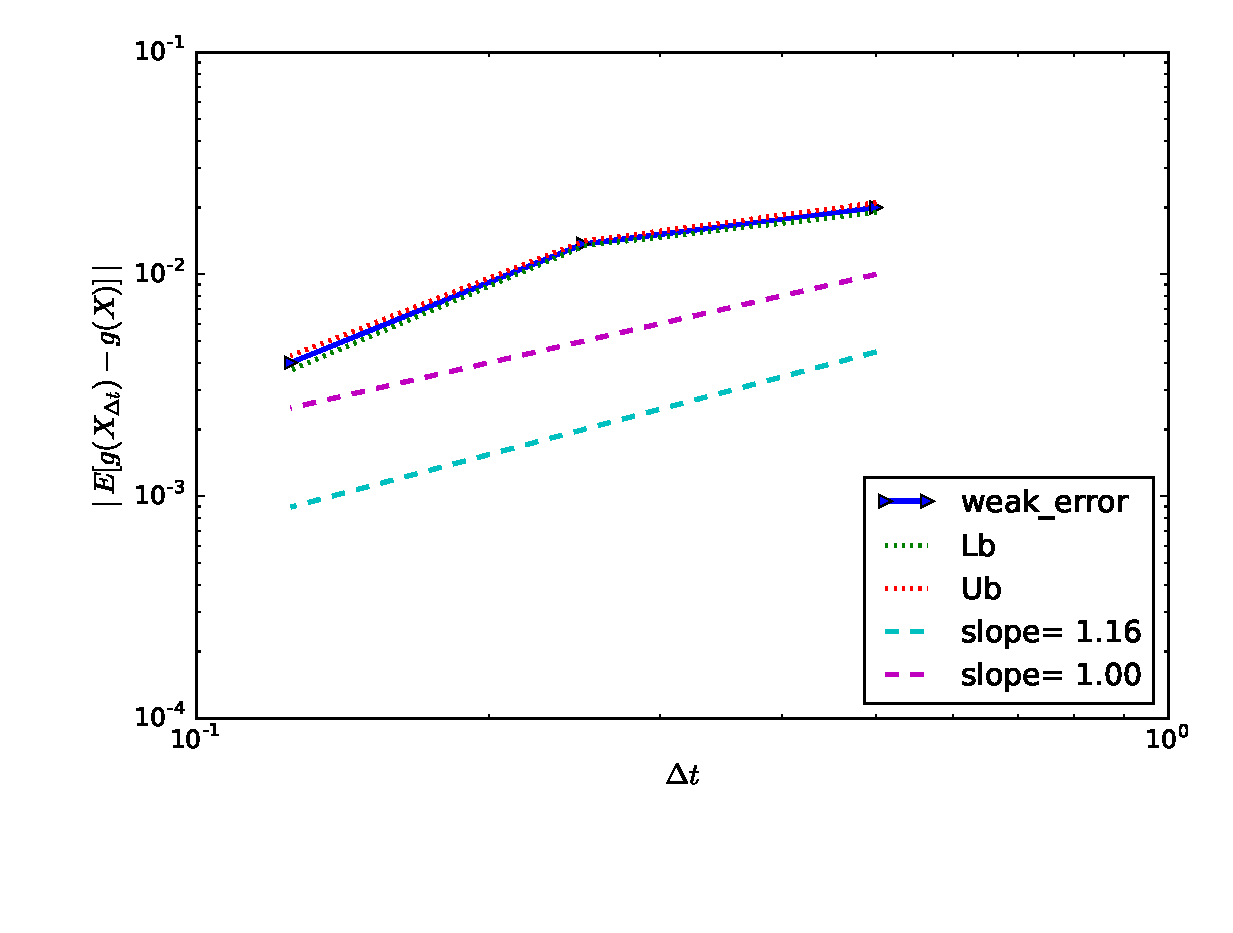
\includegraphics[width=0.4\linewidth]{./figures/basket_call_4d_time_stepping/weak_convergence/weak_convergence_order_basket_option_4d_relative_M_4_10_6_beta_256}

	\caption{The convergence of the relative weak error  $\mathcal{E}_B(N)$ defined in \ref{eq:total_error}, for the $4$-dimensional basket call option with  a number of Laguerre  quadrature points  $\beta=512$ and number of samples for MC $M=4 \times 10^6$. The upper and lower bounds are $95\%$ confidence intervals.}
	\label{fig:Weak_rate_4_dim_basket}
\end{figure}
\FloatBarrier

\FloatBarrier
\begin{table}[h!]
	\centering
	\begin{tabular}{l*{6}{c}r}
		\toprule[1.5pt]
	Method & & Steps  & &     \\
	\hline
           & $2$ & $4$ & $8$   \\
		\hline
		MISC   &  $\underset{(0.02,0.02)}{\mathbf{0.04}}$ & $\underset{(0.013,0.014)}{\mathbf{0.027}}$ & $\underset{(0.004,0.004)}{\mathbf{0.008}}$   \\

		\hline		
			MC +root finding   &  $\underset{(0.02,0.02)}{\mathbf{0.04}}$ & $\underset{(0.013,0.012)}{\mathbf{0.025}}$ & $\underset{(0.004,0.004)}{\mathbf{0.008}}$  \\
			M(\# MC samples)   & $10^3$   &  $3 \times 10^3$ &  $3 \times 10^4$  \\	
		\hline	
				MC   &  $\underset{(0.02,0.02)}{\mathbf{0.04}}$ & $\underset{(0.013,0.013)}{\mathbf{0.026}}$ & $\underset{(0.004,0.004)}{\mathbf{0.008}}$   \\	
				M(\# MC samples)   &$2 \times 10^4$  & $7 \times 10^4 $  &  $7 \times 10^5 $ \\	
		
			\bottomrule[1.25pt]
	\end{tabular}
	\caption{Total relative  error of MISC, with different tolerances, and MC to compute $4$-dimensional basket call option price for different number of time steps, without Richardson extrapolation. The values between parentheses correspond to the different errors contributing to the total relative error: for MISC we report the bias and quadrature errors and for MC we report the bias and the statistical errors. The number of MC samples,$ M$, is chosen to satisfy \eqref{optimal_number_samples}.}
	\label{Total error of MISC and MC to compute 4 dim basket  Call option price of the different tolerances for different number of time steps, without Richardson extrapolation. The numbers between parentheses are the corresponding absolute errors.}
\end{table}
\FloatBarrier




\begin{table}[h!]
	\centering
	\begin{tabular}{l*{6}{c}r}
		\toprule[1.5pt]
	Method & & Steps  & &     \\
	\hline
	         & $2$ & $4$ & $8$    \\
		\hline
		MISC & $4$  & $13$ & $22$     \\
			MC  +root finding  & $222$&  $730$&  $10541$   \\
				MC  &   $10$& $44$ &   $603$ \\
		\bottomrule[1.25pt]
	\end{tabular}
	\caption{Comparison of the computational time of  MC and MISC, used to compute $4$-dimensional basket call option price  for different number of time steps, without Richardson extrapolation. The average computational time of MC is computed over $10$ runs.}
	\label{Comparsion of the computational time of  MC and MISC, used to compute 4 dim basket Call option price  for different number of time steps, without Richardson extrapolation}
\end{table}


\FloatBarrier


	\begin{figure}[h!]
\centering
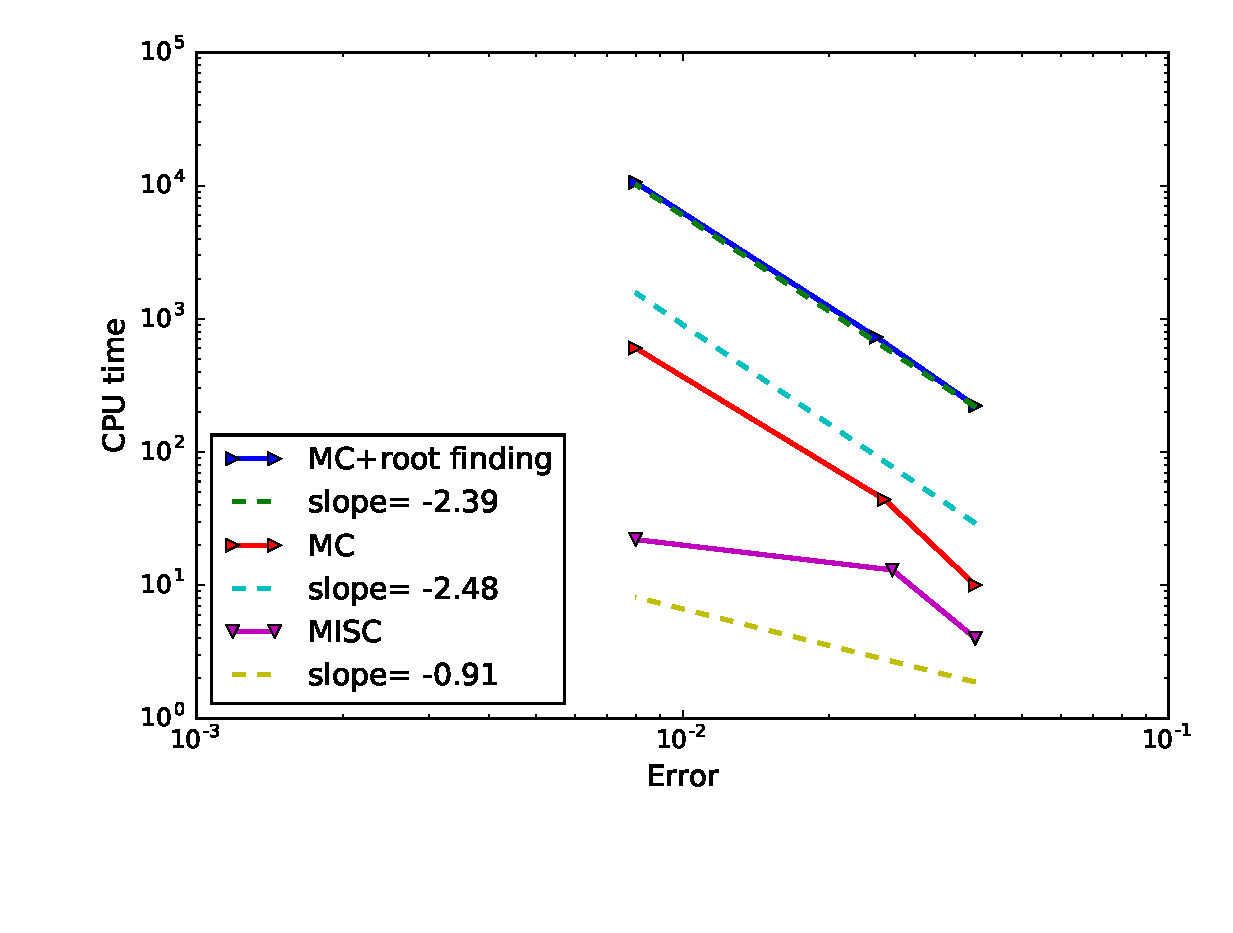
\includegraphics[width=0.4\linewidth]{./figures/basket_call_4d_time_stepping/complexity_rates/error_vs_time}

\caption{Computational work comparison for MISC and MC methods, for the case of $4$-dimensional basket call option. This plot shows that to achieve a relative error below $1\%$, MISC outperforms significantly MC method in terms of computational time.}
\label{fig:Complexity plot for MC and MISC , 4 dim basket call non rich}
\end{figure}


\FloatBarrier

%\subsection{The call on max  option under GBM}\label{sec:The best call option  under GBM}
%The fourth example that we consider is  the European rainbow option under BBM model and in particular the call on max option whose payoff is given by
%\begin{align}\label{eq:max_call_option}
%\max\left( \max\left(S_1,\dots,S_d\right)-K,0 \right).
%\end{align}
%
%We start here by the two dimensional call on max option under the GBM model. The discretization of the assets is the same as given in  \eqref{eq:discrete_rep_2} and \eqref{eq: incremental functions}, where we use the same transformation as in Section \ref{sec:Step $1$: Numerical smoothing}. This implies that, in order to determine $Y^{\ast}_1$, we need to solve
%\begin{align}
%	x=\max\left(X_0^{(1)}  \prod_{i=0}^{N-1} g_i^{(1)}(Y^{\ast}_1(x),\mathbf{Y}_{-1}),X_0^{(2)}  \prod_{i=0}^{N-1} g_i^{(2)}(Y^{\ast}_1(x),\mathbf{Y}_{-1})\right)
%\end{align}
%
%
%For illustration, we consider the example with parameters:  $S_0^{1,2}=K=100$, $\sigma_{1,2}=0.4$, $\rho=0.3$, $T=1$, and  $r=0$, the reference value for those parameters  is  $26.40$.




\subsection{Options under the discretized the Heston model}
In this section, we consider  testing options under the discretized Heston model \cite{heston1993closed,broadie2006exact,kahl2006fast,andersen2007efficient} whose dynamics are given by
\begin{align}\label{eq:dynamics Heston}
dS_t&=\mu S_t dt+\sqrt{v_t}S_t dW_t^S= \mu S_t dt+ \rho\sqrt{v_t}S_t dW_t^v+ \sqrt{1-\rho^2} \sqrt{v_t}S_t dW_t \nonumber\\
dv_t&=\kappa (\theta-v_t)dt+\xi \sqrt{v_t} dW_t^v\COMMA
\end{align}
where 

\begin{itemize}
\item $S_t$ is the price of the asset, $v_t$ the instantaneous variance, given as  a CIR process.
\item $W_{t}^{S},W_{t}^{v}$ are correlated Wiener processes with correlation $\rho$.
\item $\mu$  is the rate of return of the asset.
\item $\theta$ is  the mean  variance.
\item $\kappa$ is the rate at which $v_t$ reverts to $\theta$.
\item $\xi$ is the volatility of the volatility, and determines the variance of $v_t$.
\end{itemize}
%We also consider cases where the parameters fulfill the Feller condition
%\begin{align*}
%2 \kappa \theta >\xi^2,
%\end{align*}
%implying  that the process $v_t$ is strictly positive.

\subsubsection{Discretization of Heston model}
Given that the SDE for the asset path is now dependent  upon the solution of the second volatility SDE in \eqref{eq:dynamics Heston}, it is necessary to simulate the volatility process first and then utilize this "volatility path" in order to simulate the asset path. In the case of the original GBM SDE it is possible to use It\^o's Lemma to directly solve for $S_t$. However, we are unable to utilize that procedure here and must use a numerical approximation in order to obtain both paths. 

Applying Forward Euler scheme to descretize \ref{eq:dynamics Heston} implies 
\begin{align}\label{eq:FE_Heston_discrete}
S_{t+\Delta t}&= S_t +\mu S_t \Delta t+\sqrt{v_t \Delta t}S_t Z_s \nonumber\\
v_{t+\Delta t}&=f_1(v_t)+\kappa (\theta-f_2(v_t)) \Delta t+\xi \sqrt{f_3(v_t) \Delta t} Z_v \nonumber\\
v_{t+\Delta t}&=f_3(v_{t+\Delta t}4) \COMMA
\end{align}
where $Z_s$ and $Z_v$  are two correlated standard normal variables with correlation $\rho$, such that $Z_s=\rho Z_v+\sqrt{1-\rho^2} Z_t$, and to avoid problems with negative values of $\sqrt{v_t}$, we introduce $f_1, f_2$, and $f_3$, which with different choices implies different schemes used in the literature 

\FloatBarrier
\begin{table}[h!]
	\centering
	\begin{tabular}{l*{6}{c}r}
		\toprule[1.5pt]
	Scheme &  $f_1$& $f_2$  & $f_3$     \\
	\hline
	full truncation scheme & $v_t$ &  $v_t^+$&$v_t^+$\\
	Partial truncation scheme & $v_t$ &  $v_t$&$v_t^+$\\
	The reflection scheme  &$\abs{v_t}$ & $\abs{v_t}$& $\abs{v_t}$\\
			\bottomrule[1.25pt]
	\end{tabular}
	\label{Numerical schemes for CIR process}
\end{table}
\FloatBarrier
where  $v_t^+=\max(0,v_t)$.

The literature \cite{lord2010comparison} suggest that the Full Truncation method is the "best" option and so this is what we will utilize here. 

\subsubsection{European call option  under the discretized the Heston model }

The  first example that we test under the Heston model is the single European call option with parameters: $S_0=K=100$, $v_0=0.04$, $\mu=0$, $\kappa=5$, $\theta=0.04$, $\xi=0.1$ and $\rho=-0.9$. The reference value in this case is $7.5789$. For solving the root finding problem we follow similar approach to the one in Section \ref{sec:Determining the kink location} with substituting $\sigma$ with $\sqrt{v_i}$ in $f_i$.

Figure \ref{fig:Weak_rate_heston_single_call} shows the estimated   weak error  for the case without Richardson extrapolation.

\FloatBarrier
\begin{figure}[h!]
		\centering
		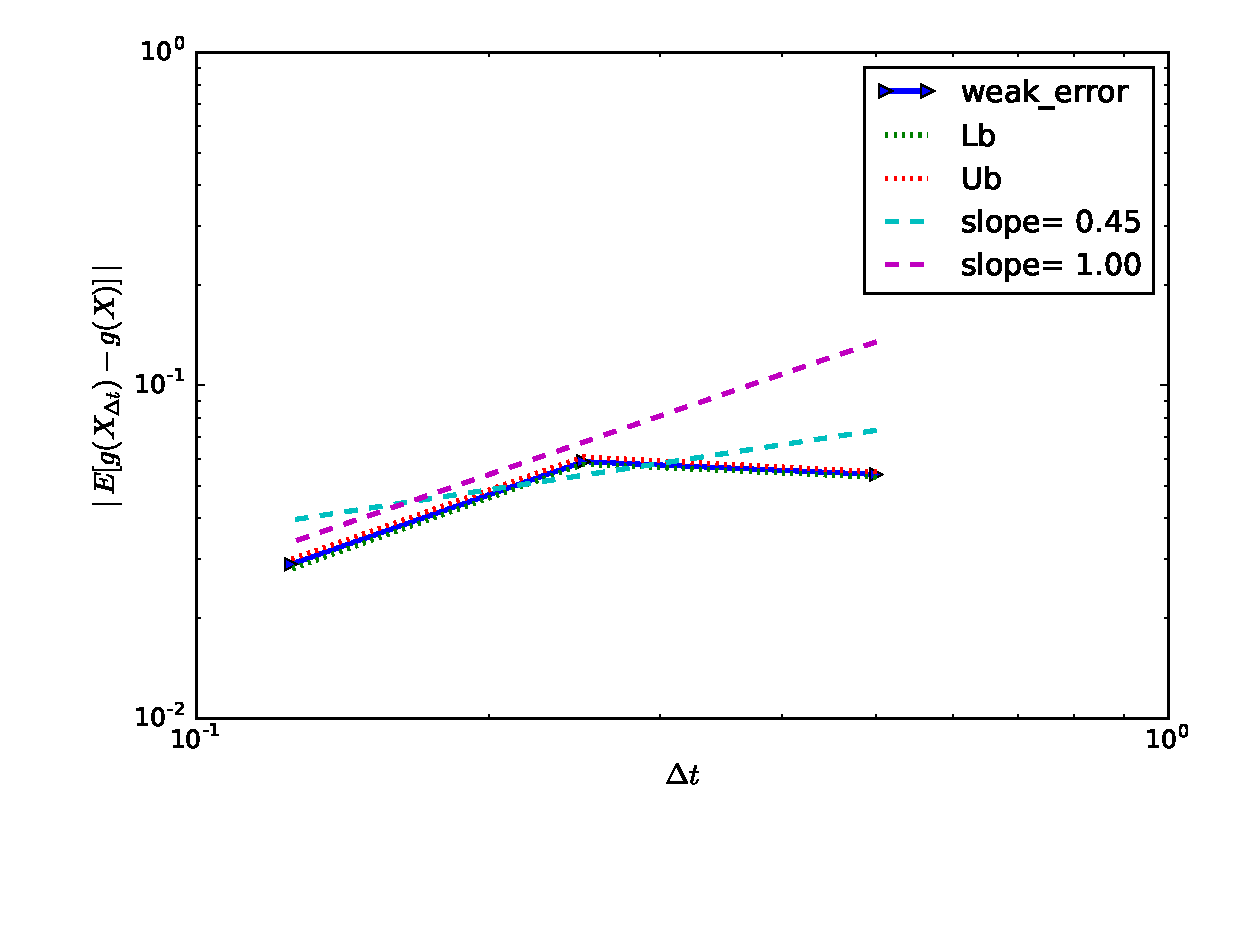
\includegraphics[width=0.4\linewidth]{./figures/Heston_single_call/weak_convergence/weak_convergence_order_single_call_option_heston_relative_M_4_10_6_beta_512}
	\caption{The convergence of the relative weak error  $\mathcal{E}_B(N)$ defined in \ref{eq:total_error}, for the single call option under the Heston model with  a number of Laguerre  quadrature points  $\beta=512$ and number of samples for MC $M=4 \times 10^6$. The upper and lower bounds are $95\%$ confidence intervals.}
	\label{fig:Weak_rate_heston_single_call}
\end{figure}
\FloatBarrier

\subsubsection{Basket call option under the discretized the Heston model }

\subsubsection{Call on max option under the discretized the Heston model }

